\chapter{Compton camera application for ion beam therapy monitoring}\label{chap::4}

The results presented in this chapter have been submitted for publication on the journal \textit{Physics in Medicine and Biology}.

\vfill

\minitoc

\newpage

\glsresetall
\glsunset{clarys} 

\section{Introduction}\label{chap4::sec::Intro}
Ion beam therapy is a cancer treatment technique which is rapidly gaining importance in the global tumor therapy panorama. In addition to the already operational 70 clinical facilities, with more than 175000 patients already treated by the end of 2017, several new centers have been designed and approved for construction worldwide~\parencite{PTCOG2017}. The favorable feature of this treatment technique is connected to the peculiar energy deposition profile of charged particles as a function of depth in matter. As first observed by Bragg~\parencite{Bragg1904}, the depth-dose profile of charged particles shows a maximum close to the end of their range in matter; in addition to this, a strong enhancement of the \gls{rbe} is observed for ions heavier than protons in the region of the Bragg peak~\parencite{Elsasser2004, Weyrather1999}, which further enhances the dose ratio between target and healthy tissues.

The maximum of the dose is deposited in the Bragg peak region in the patient and must be tuned to cover the target volume (defined via \gls{ct} scan) and, at the same time, spare the surrounding healthy tissues. Treatment planning and delivery uncertainties limit the tumour targeting capabilities, like uncertainties in the material composition determination, \gls{ct} units conversion to ion stopping power, patient mis-positioning, organ motion or morphological changes between treatment fractions. These uncertainties force the clinicians to fix relatively large safety margins around the planned treatment volume, up to 3.5\% + 3 mm~\parencite{Paganetti2012}. Ion-range verification is one of the conditions required for a broader usage of ion beam therapy and for its further development. With the goal of fully exploiting the ion beam therapy dosimetric potential, the monitoring should be in real-time and ideally in 3 dimensions, in order to detect important deviations between the planned and delivered dose to the target volume or to surrounding organs, in particular in case of proximity to \gls{oar}. This capability would allow for a reduction of the above mentioned safety margins and for a better tumor targeting; in addition to this, it could permit the use of new irradiation fields with \gls{oar} downstream with respect to the tumor position~\parencite{Knopf2013}.   

Several range verification techniques have been considered worldwide for twenty years. Most of them rely on the detection of secondary radiation generated during the slowing down process of incident ions, in particular during nuclear reactions. Among theses secondary radiations, positron emitters have been deeply studied in order to exploit \gls{pet} machines for treatment monitoring. The only available and functional range monitoring systems in a clinical center are based on this technique~\parencite{Enghardt2004, Yamaya2018}, which is anyway affected by physical and technical limitations~\parencite{Parodi2015}.

In addition to positron annihilation products, the relaxation of excited nuclei also produces secondary photons in a wide energy range, between some hundreds of keV till about 8-10~MeV. After the first idea proposal published in 2003~\parencite{Stichelbaut2003}, these secondary products of particle treatment have been deeply investigated and the correlation of this gamma radiation to the ion depth-dose profile has been confirmed by several research groups, starting from~\cite{Min2006} for protons and~\cite{Testa2008} for carbon ions. The so-called \gls{pg}-rays have the advantage to be emitted almost instantaneously after the beam interaction in the tissue, making them more adapted than \gls{pet} 511~keV gammas for real-time monitoring. Moreover, as shown in~\parencite{Robert2013}, the emission rate is comparable or superior to the one of the annihilation gammas for both protons and carbon beams. Consequently, different techniques have been proposed to exploit this signal for treatment monitoring purpose, with the related detection systems. More details on \gls{pg} monitoring can be found in chapter~\ref{chap::2}.
In the same chapter, in section~\ref{chap2::sec::PGdevices}, the methods and devices developed for the detection of \gls{pg} rays with the purpose of monitoring the ion range during particle therapy treatments are described. In particular, Compton camera prototypes have been studied and developed by several groups.
Several sources of uncertainty and signal background are connected to the Compton camera detection method. The reported Compton kinematics formula (equation~\ref{chap2::eq::ComptonAperture}) assumes valid the relation in equation~\ref{chap4::eq::energy_equation}:
 \begin{equation}
E_{0} = E_{1}+E_{2}.
\label{chap4::eq::energy_equation}
\end{equation} 
where $(E_{0}$ is the energy of the incident photon,  $(E_{1}$ and $(E_{2}$ are the energies deposited by the detected photon in scatterer and absorber, respectively.
Since the initial photon energy is not known \textit{a priori}, a complete photon energy absorption is needed for the cone calculation, or at least three photon interactions are required in a single event. An under-estimation of the total initial energy (caused by a photon non-complete absorption in the absorber section or by the Compton electron escape from the scatterer section), leads to a mis-estimation of the Compton angle, so to a Compton cone reconstruction uncertainty. If triple scattered photons are selected, the initial photon energy can be calculated analytically so that a complete absorption is not mandatory~\parencite{Kurfess2000}. In addition to this, the Compton formula considers the Compton scattering electron initially at rest, and its energy configuration creates a blur in the Compton angle reconstruction, resulting in the already cited Doppler broadening effect~\parencite{Ordonez1997}. Furthermore, the detection principle is based on time coincidences between the two detector sections, therefore the time structure of the incoming particles plays an important role. The final image accuracy suffers from random coincidences generated by two prompt gammas interacting within the same time window or by contamination of secondaries, mainly neutrons and protons. The effect of random coincidences can be reduced by high detector time resolution or background rejection methods~\parencite{Draeger2017}. Energy selections can be applied to the collected coincidences~\parencite{Polf2009, Hilaire2016} or the homogeneous neutron background can be reduced via time-of-flight information~\parencite{Testa2010}.

Ortega and colleagues~\parencite{Ortega2015} presented a detailed analysis of the noise sources for Compton imaging in proton therapy monitoring, and the clinical application of this method for detecting range shifts was tested for the setup under development in Valencia. The simulation study showed the relative expected rate of prompt gammas and neutrons, and the resulting rate of random coincidences ranging from 19 \% to more than 60 \% depending on the beam energy and the coincidence time window. This amount of fake events leads to complex reconstruction scenarios, where the identification of a 3~mm range shift is not clear for all cases.

Starting from these results, we studied with Monte Carlo simulations the Compton camera prototype developed by the \gls{clarys} collaboration based on semiconductor and scintillator detectors (see chapter~\ref{chap::3} and~\cite{Krimmer2015, Fontana2018}).
The camera performance is studied with respect to the gamma energy in the prompt gamma energy range. Furthermore, the feasibility of its clinical application as depth-dose profile monitor during ion beam therapy clinical treatment is analyzed. After a preliminary study with point-like gamma sources irradiation focused on detector efficiency measurements as a function of the source position and gamma energy, clinical proton and carbon beams impinging on an homogeneous \gls{pmma} phantom are simulated to reproduce treatment conditions and analyze the prompt gamma detection resulting scenario. The ratio between true and random coincidences is studied as a function of the beam intensity. Two kinds of reconstruction algorithms, a line-cone analytic method and a \gls{mlem} iterative one, are applied to the collected data in order to compare the imaging results. Finally, the precision with which the dose profile fall-off can be detected with the Compton camera is reported.   


\section{Material and methods}\label{chap4::sec::MatMet}

\subsection{Simulation setup}\label{chap4::subsec::SimuSetup}

The monitoring system modeled in this simulation work is the Compton camera prototype under development within our collaboration. The detectors detailed characteristics can be found in chapter~\ref{chap::3}, and are here briefly recalled.\\
%Like most of the Compton camera devices, the CLaRyS prototype includes a scatterer and an absorber. 
The scatterer consists of seven parallel planes of silicon detectors (\glspl{dssd}), $9\times9\times0.2$~cm$^3$, with 1~cm distance between the centers of two neighboring planes, while the absorber is composed of an array of $10\times10$ \gls{bgo} blocks ($3.5\times3.5\times3.0$~cm$^3$ each) placed behind the silicon layers at a distance which can be tuned according to the requirements.

\begin{figure}	
  \centering
  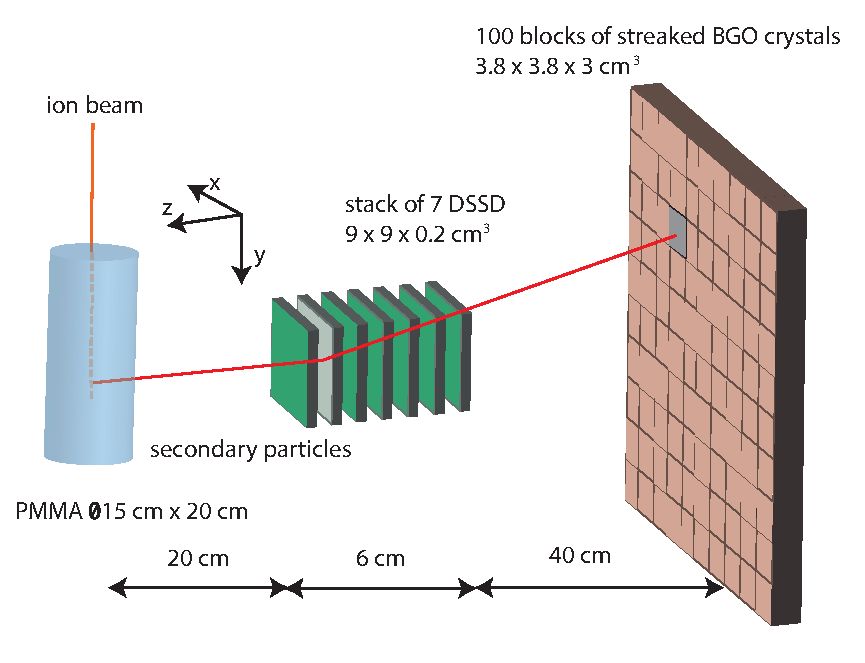
\includegraphics[width=0.7\textwidth]{03_GraphicFiles/chapter4_HTsimu/Compton_Camera_hadontherapy_PMMA_Cylinder_EN.pdf}
  \caption{Scheme of the simulation setup (not at scale): a \gls{pmma} cylindrical phantom is set in front of the Compton camera prototype. The Compton camera is composed of a stack of 7 \glspl{dssd} (scatterer) and a plane of 100 single \gls{bgo} blocks. The set distances are realistic for clinical conditions. This geometrical configuration has been used for all the simulations presented in this work.}
  \label{chap4::fig::fig_setup_CC_simulation_Hadronth}
\end{figure}

The silicon detectors have a strip pitch of 1.4~mm, for a total of 64 strips per side (double-sided readout based on electron and hole pairs collection). 
Regarding the \gls{bgo} blocks, their entrance surface is streaked in a 8$\times$8 matrix of pseudo-pixels, $4.4\times4.4$~mm$^{2}$ size, and the readout is performed via 4 \gls{pm} tubes. The position reconstruction is achieved via Anger logic.

A scheme of the simulation setup is given in \figurename~\ref{chap4::fig::fig_setup_CC_simulation_Hadronth}. The ion beam interacts with a cylindrical \gls{pmma} phantom (15~cm diameter and 20~cm length) placed in front of the Compton camera as target. It is placed 20~cm far from the first silicon plane (center-to-center distance) which seems a realistic distance in clinical conditions. The distance between the last silicon layer and the absorber array (center-to-center) is set to 40~cm in order to enable \gls{tof} measurements (see section~\ref{chap4::subsec::MatMeth::TOF_Ecut}).

The silicon detector strips are not reproduced in the simulation code, and the spatial resolution in the detector plane is set to 0.9~mm \gls{fwhm} at the reference energy of 1~MeV, according to preliminary measurements performed on smaller detector prototypes. In the plane of the detectors (xy in \figurename~\ref{chap4::fig::fig_setup_CC_simulation_Hadronth}), interactions are defined as localized energy deposits, and the events presenting multiple hits separated by a distance beyond 3-strip equivalent are rejected. For the accepted multiple-hit interactions, the interaction position in the detector plane is defined as the center of gravity of the hits, weighted with the hit energy deposit. Concerning the direction perpendicular to the detector plane (z axis in \figurename~\ref{chap4::fig::fig_setup_CC_simulation_Hadronth}), the interaction position is set to the center of the involved silicon plane. A mono-block crystal is simulated for the absorber for simplicity. The events are selected to be limited to a single block component based on the interaction localization, and, as for the scatterer layers, the interaction position is reconstructed via center of gravity calculation if multiple interactions occur within the same block. An uncertainty contribution, randomly extracted from a Gaussian of 5~mm \gls{fwhm} (corresponding to an overestimation of the geometrical resolution given by the pseudo-pixel matrix, set to reproduce not yet tested experimental conditions), is added to the reconstructed position to mimic the pseudo-pixel-based readout. For what concerns the z direction, given the fact that the employed \gls{bgo} blocks have not \gls{doi} reconstruction capabilities, the interaction position is fixed to the center of the mono-block crystal.

The energy resolution of the silicon detector is set to 5~keV \gls{fwhm} for an energy deposit of 200~keV according to the design expectations, and varies as a function of $\sqrt{E_{1}}$. The energy resolution of the \gls{bgo} blocks was estimated in preliminary measurements and is accordingly set to 20\% \gls{fwhm} at the reference energy of 667~keV (a $^{137}$Cs source has been used for the measurements).

The time resolution has been set to 15.0~ns \gls{fwhm} for the silicon slabs and to 3.0~ns \gls{fwhm} for the \gls{bgo} blocks, according to preliminary measurements performed on test detector modules at the \gls{ganil} center in France.

The detector resolutions play an important role in the Compton camera performances. The spatial resolution of the absorber influences the position of the axis orientation of the Compton cone. The energy resolution of the scatterer determines the Compton cone aperture angle. The time resolution impacts the coincidence window between the absorber and the scatterer, and therefore the detectors ability to distinguish between true and random coincidences.

The \gls{clarys} project also includes the development of a beam tagging hodoscope, composed of scintillating fibers read out by multi-channel \glspl{pm}. This detector is used to synchronize the beam time and space structure to the \gls{pm} detection in order to tune the detection window reducing the background contamination. In addition to this, the spatial localization of the impinging beam bunch can be included in the event reconstruction algorithm to add constraints to the obtained solutions (see section~\ref{chap4::subsec::MatMeth:reconstruction}). The hodoscope is not included in the simulation, but its spatial and time resolution have to be taken into account for the \gls{tof} discrimination (see section~\ref{chap4::subsec::MatMeth::TOF_Ecut}) and events reconstruction. They are set to 1~ns and 1~mm \gls{fwhm}, respectively.\\ 
The detector's spatial, energy, and time resolutions are summarized in table~\ref{chap4::tab::table_resolution_detectors_CC_simulation_Hadronth}.

\begin{table}[!htbp]

\centering
%\begin{tabular}{>{\columncolor[gray]{0.9}}ccc}
\caption{Estimations of reachable resolutions with the detectors. Those resolutions are applied during the simulations.}
\label{chap4::tab::table_resolution_detectors_CC_simulation_Hadronth}
\begin{tabular}{cccc}
\toprule
\rowcolor{myColorMainA!20} 
\textbf{Resolution (FWHM) at 1~MeV} & \textbf{Scatterer} & \textbf{Absorber} & \textbf{Hodoscope}\\
\midrule
\textbf{spatial [mm]	}			 &     0.9		 &  5 &	 1\\
%\hline
\textbf{energy}				&	5~keV		&  17~\%	&	/\\
%\hline
\textbf{timing [ns]}	        		&	15			&	3 	&  1\\
\bottomrule
\end{tabular}
\end{table}
    
The Monte Carlo simulation is performed with the Geant4 toolkit, version 9.6.02. 
%Geant4 has been developed at CERN %(Conseil europ\'{e}en pour la recherche nucl\'{e}aire) for high energy physics experiments, but it has been shown that it can be used for ion beam therapy studies \cite{cirrone_hadrontherapy_2011,toshito_new_2010}. 
%Some improvements are still needed in order to extend the hadronic models to low energy applications~\cite{dedes_assessment_2014, Pinto:2016aa}.
The particle interactions in matter are described in this work by means of the models listed in table~\ref{chap4::tab::physlist_ion}. Additionally, the Doppler broadening and the photon polarization effects are included.
 
\begin{table}
\centering
\caption{Hadronic models used in the Geant4 simulations.}
\label{chap4::tab::physlist_ion}
\resizebox{\textwidth}{!}{%
\begin{tabular} {cccc}
\toprule
\rowcolor{myColorMainA!20} 
\textbf{Process} & \textbf{Protons} & \textbf{Ions} & \textbf{Neutrons} \\ 
\midrule
\textbf{Electromagnetic} & \multicolumn{3}{c}{standard$_{\mathrm{option3}}$} \\ %\hline
\textbf{Inelastic} & G4BinaryCascade & G4QMDReaction  &  G4BinaryCascade  \\ 
 & & (G4IonsShenCrossSection)&+ G4NeutronHPInelastic ($<$19~MeV)\\ %\hline
\textbf{Elastic} & G4LElastic & G4LElastic & G4LElastic + G4NeutronHPElastic ($<$19~MeV)\\ %\hline
\textbf{Fission} & / & / & G4LFission + G4NeutronHPFission($<$19~MeV) \\ %\hline
\textbf{Capture} & / & / & G4LCapture +  G4NeutronHPCapture ($<$19~MeV) \\ %\hline
\textbf{Radioactivedecay} & / & G4Radioactivedecay & / \\
\bottomrule
\end{tabular}}
\end{table}


\subsection{Beam structure}\label{chap4::subsec::BeamModeling}
\subsubsection{Beam structure measurements at HIT}\label{chap4::subsubsec::beam_measurement}
Our group performed a set of measurements to characterize the beam time structure of the synchrotron installed at \gls{hit}, Germany~\parencite{Peters2008}. This set of measurements extends the results reported in~\cite{Peters2008} and is then used to reproduce a realistic beam in the simulation.\\
The beam characterization has been performed for 200~MeV/u and 400~MeV/u primary ion energy with a two-fiber hodoscope (basic prototype of the one at present under development - see chapter~\ref{chap::3}) and the spill signal was given by the accelerator. \figurename~\ref{chap4::fig::fig_HIT_timeStruct} shows the results for carbon ions at 400~MeV/u. The pulses have a spill period of 150.2~ns and each bunch is approximately 21.5~ns.
The mentioned measurements have shown that the spill phase changes during the extraction: this implies that the \gls{rf} signal from the synchrotron can not be used to trigger the pulses, so that the use of an additional beam time stamp system like the hodoscope seems required for \gls{tof} background rejection purposes.

\begin{figure} [!hbtp]	
  \centering
	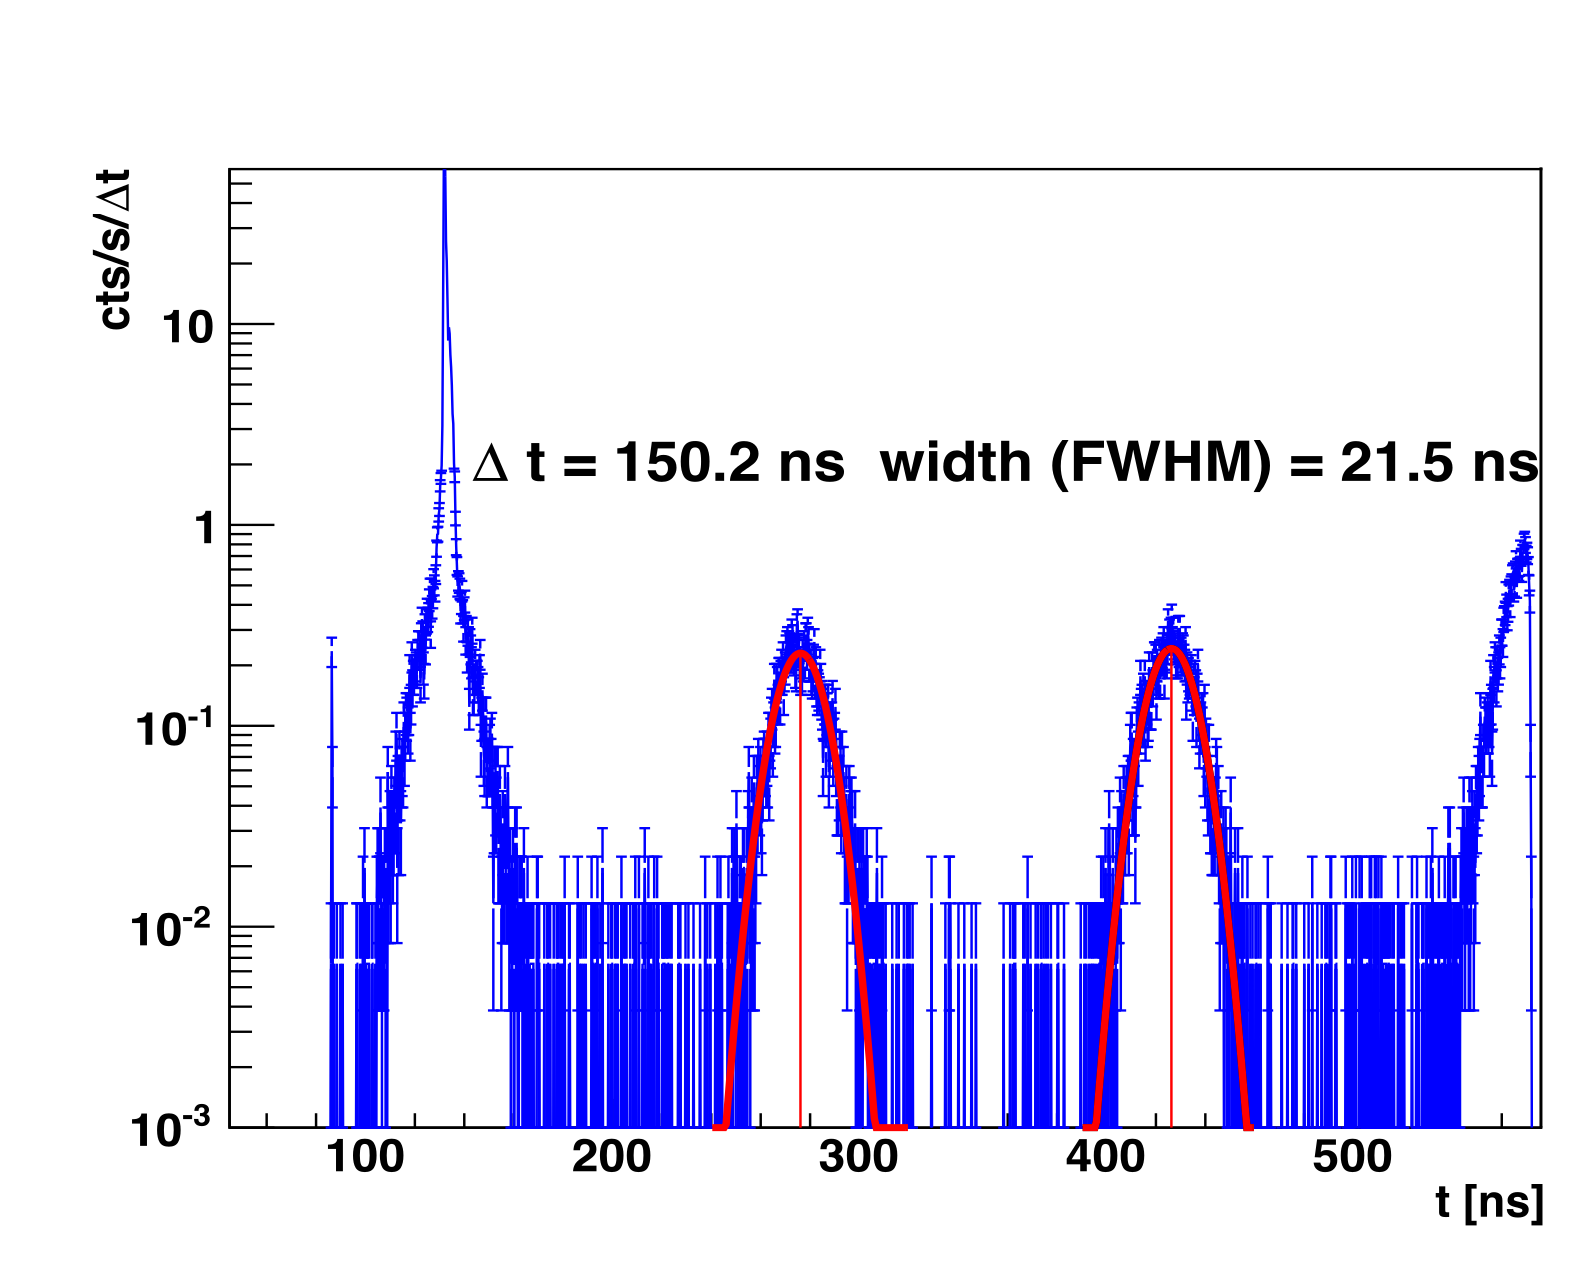
\includegraphics[width=0.6\textwidth]{03_GraphicFiles/chapter4_HTsimu/BeamTimeStruct.png} 
  \caption{Beam time micro-structure measured from a carbon ion beam at 400~MeV/u delivered at \gls{hit} (time difference between two crossed-scintillating fibers). The offset between the two fibers is arbitrarily set to 130~ns. The pulses have an extraction period of 150.2~ns and the bunches are 21.5~ns \gls{fwhm}.  On the x axis the time has been measured with a two-scintillating-fiber hodoscope, with 1~ns \gls{fwhm} time resolution.}
  \label{chap4::fig::fig_HIT_timeStruct}
\end{figure}


\subsubsection{Beam modeling}\label{chap4::subsubsec::beam_modeling}
The two main beam particles used in clinics are considered in the simulation: protons and carbon ions. The beam range of interest is 15.2~cm in the \gls{pmma} phantom, and the associated energy is 160~MeV for protons and 305~MeV/u for carbon ions.\\ 
The beam transverse dimension is modeled with a Gaussian distribution with a standard deviation of 5~mm for protons at 160~MeV and 3.5~mm for carbon ions at 305~MeV/u. The number of incident ions for a spot in \gls{pbs} mode is $10^8$ for protons (distal spot - upper intensity limit) and $10^5$ for carbon ions (average spot intensity)~\parencite{Kramer2000, Grevillot2011, Smeets2012}. In the simulation, the beam intensity is modeled by an average number of particles per bunch. The exact number of particles in each bunch is given by a random extraction from a Poisson distribution, where the mean value is the selected beam intensity.\\
The beam time structure is applied at the data analysis stage. Two different time structures have been considered for this study, related to two kinds of accelerators used in clinical practice: the \gls{iba} C230 cyclotron for protons (used in 16 clinical centers worldwide) and the \gls{hit} synchrotron for carbon ions. For protons at 160 MeV, the primary particles are grouped in bunches of 2~ns (this value may vary also according to the distance between the cyclotron and the treatment room, and energy spread selection) at a frequency of 106~MHz (9.42~ns)~\parencite{Roellinghoff2014}. The clinical beam intensity is 3.2~nA which corresponds to about 200 protons per bunch. Concerning the carbon ion beam at 305~MeV/u, the simulated time structure refers to the measurements presented in section~\ref{chap4::subsubsec::beam_measurement}. We used 30~ns duration bunches at a frequency of 5.9~MHz (170~ns period). The clinical beam intensity for carbon ions is $5\times10^7$~ions/s during extraction, corresponding to about 9~ions per bunch. The macro-structure (~50\% duty cycle with [1,5]~ns period) is not considered. 

The coincidence window (between scatterer and absorber events) is set to 40~ns, centered on each absorber detected interaction. This value is adapted to the detectors time resolutions. At the simulation stage, each interaction in the detector layers is collected with the related local time. The beam time structure is then applied to each single hit, and the selected coincidence window is used to retrieve scatterer-absorber coincidence events.\\ 
Table~\ref{chap4::tab::definition_beam_structure_CC_hadrontherapy_Geant4} summarizes the presented beam time structures and coincidence reconstruction features.

\begin{table} [!htbp]
\centering
\caption{Description of the two beam structures studied: the \gls{iba} cyclotron C230 for protons and the synchrotron installed at the \gls{hit} center in Germany for carbon ions. The macro-structure of the synchrotron, at the second time scale, is not considered here. The beam structures are applied to the simulation data.}
\label{chap4::tab::definition_beam_structure_CC_hadrontherapy_Geant4}
\setlength{\tabcolsep}{2pt}
\resizebox{\textwidth}{!}{%
\begin{tabular}{c|c|cc}
%\cline{2-4}
\toprule
\rowcolor{myColorMainA!20} 
		\multicolumn{2}{c}{ }		 & 					\textbf{Protons} & \textbf{Carbon ions}\\ 
\midrule
%\cline{2-4}%\hline
\multirow{3}{*}{\textbf{Clinical features}}		&	Facility	& \gls{iba} Cyclotron C230 &   Synchrotron at \gls{hit}\\
											& Clinical intensity& $  2\times10^{10}$ p/s  & $  5\times10^{7}$ ions/s\\
											& Energy 			&160~MeV 			&    305~MeV/u\\
%\cline{2-4}%
\midrule
\multirow{3}{*}{\textbf{Beam structure}}	&	Bunch time [ns]	& 3.2				&  30\\
											& Period [ns]		&   9.4 				& 170\\
											& Primaries/bunch 	&217 			& 9\\
%\cline{2-4}%
\midrule
\multirow{2}{*}{\textbf{Detectors}}						& Coincidence window [ns]		& 40 	&  40 \\
											&Time resolution (FWHM) [ns] & \multicolumn{2}{c}{Si: 15 and BGO: 3}\\
\bottomrule
\end{tabular}}
\end{table}



%\newpage
%---------------------------------------------------------------
%---------------------------------------------------------------
\subsection{Compton camera events}\label{chap4::subsec::MatMeth::events}

The Compton detection principle is based on the time coincidence of at least one scatterer and one absorber gamma interaction, where an interaction is defined as an energy deposit in a detector module, with the spatial selections detailed in section~\ref{chap4::subsec::SimuSetup}. As discussed in section~\ref{chap4::subsec::BeamModeling}, the coincidence reconstruction relies on a defined time window, fixed according to the detector resolution. In a simulation environment, different kinds of coincidence events can be distinguished and studied: 
\begin{itemize}
\item[-] real coincidences: created by a single photon first interacting in the scatterer stack and then in the absorber block array;
\item[-] quasi-simultaneous interaction of two secondary particles;
\item[-] double interaction of the same particle, not a photon (e.g. protons, neutrons).
\end{itemize}
As described in section~\ref{chap4::subsec::SimuSetup}, the simulation setup selects events with absorber interactions limited to a single \gls{bgo} block.
Concerning the scatterer section, among the real coincidences, three different kinds of events can be identified:
\begin{itemize}
\item[-] single Compton interaction in one silicon layer;
\item[-] multiple gamma interactions in more than one silicon layers;
\item[-] electron escape events.
\end{itemize}
As mentioned in the introduction, events involving more than one photon interaction in the scatterer layers are advantageous since the total absorption of the detected prompt gamma is not required to reconstruct the Compton cone. However, the actual selection of such kind of events with respect to background interactions in real conditions is hardly achievable.

On the other hand, electron escape events can be in principle identified and exploited. They are characterized by two or more scatterer layers involved: if the first Compton interaction in one layer provides enough energy to the recoil electron, it can escape the silicon plane and be detected by one (or more), neighboring planes. Thus, such events can be identified by the electron tracking, and carry additional information with respect to a Compton interaction with no electron escape. The electron tracking allows to reduce the reconstructed Compton cone to an arch of the cone, by the overlap of the cone with the electron tracking plane.      

\subsection{TOF and energy based data selection}\label{chap4::subsec::MatMeth::TOF_Ecut}

In an experiment the collected data are affected by a certain number of the so-called random coincidences, which cannot be experimentally distinguished from true coincidences, from the timing coincidence point of view. Such a background level depends on the detector time resolutions, the fixed time coincidence window and the beam time structure, the phantom composition and the camera prototype setup.
In addition to this, the prompt gamma measurement is contaminated by other secondary particles (mainly massive and charged particles like protons and neutrons, but also electrons in the low energy regime), produced by the interaction of the primary particles with the patient/phantom. In \figurename~\ref{chap4::fig::coincidence_CC_simulation_Hadronth}, a schematic view of the different kinds of possible coincidences is presented.

\begin{figure}
  \centering
  %\includegraphics[width=0.9\textwidth]{03_GraphicFiles/chapter4_HTsimu/Schema_coincidence_EN.eps}
  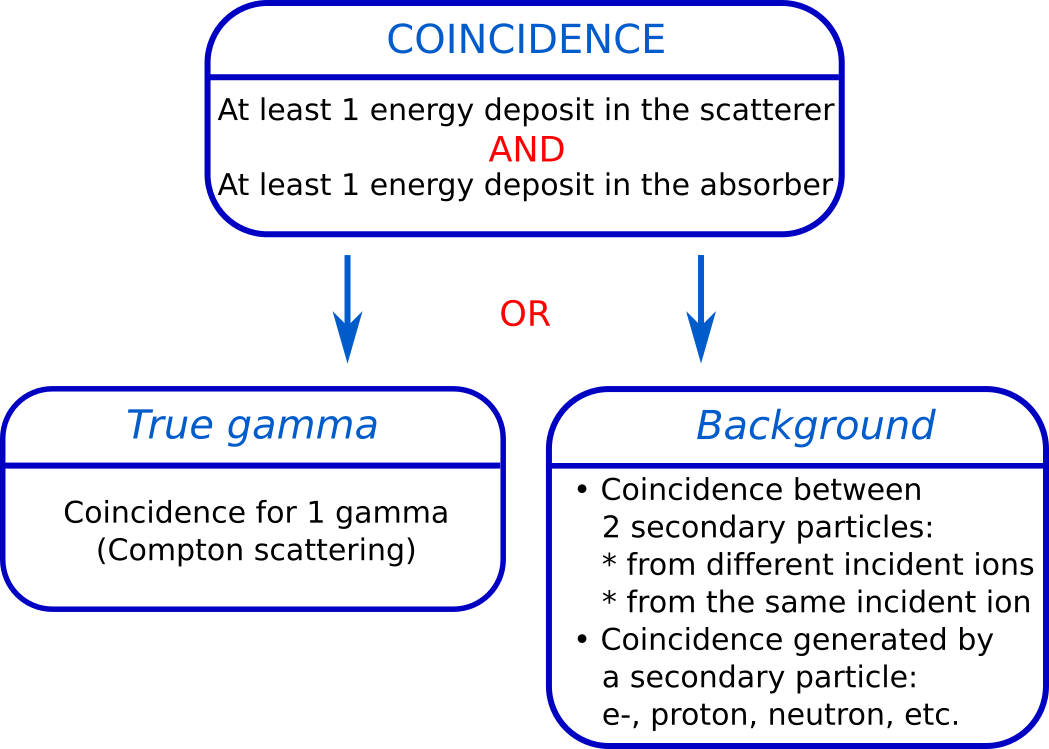
\includegraphics[width=0.9\textwidth]{03_GraphicFiles/chapter4_HTsimu/coinc_scheme.png}
  \caption{Diagram showing the different definitions of coincidences in the Compton camera. The energy deposits are selected in the silicon scatterer to be limited to neighboring strips (3 strips maximum), and in the absorber blocks the events are selected to be limited to a single block.}
 \label{chap4::fig::coincidence_CC_simulation_Hadronth}
\end{figure}

Ad-hoc filtering methods are applied to reduce the above described contamination.

\begin{itemize}
\item Time-Of-Flight: it has been demonstrated that a time-of-flight discrimination is possible and effective in reducing the background generated by massive particles interactions~\parencite{Testa2010}. The massive particles approach the detector at a lower speed with respect to photons. The time information provided by the hodoscope and the absorber can be combined to fix a detection time window and reject all the events outside the window. The time elapsed between the incident particle detection in the hodoscope and the secondary particle detection in the absorber is considered as the \gls{tof}. In order to define the appropriate time window, the \gls{tof} spectra of the collected events resulting from the irradiation of the \gls{pmma} target with 10$^{8}$ 160~MeV protons have been produced for true gamma coincidences and background events, taking into account the detector resolutions. The result is shown in \figurename~\ref{chap4::fig::fig_TOF_distribution_CC_simulation_Hadronth}. For this study, no time structure have been applied to the primary protons, thus only independent events have been considered. The \gls{tof} spectrum resulting from the simulation shows that:
\begin{itemize}
\item the coincidences of interest (produced by prompt-gamma rays) are included in a window between 0 and 8~ns;
\item in the \gls{tof} window a comparable amount of true coincidences and background events is observed. Since we consider only independent events, this means that such background events are due to random coincidences between two prompt gammas directly or indirectly induced by the same incident ion. The background events outside the \gls{tof} window are due to massive particle interactions in the camera.
\end{itemize}
It is worth to stress that the simulation results shown in \figurename~\ref{chap4::fig::fig_TOF_distribution_CC_simulation_Hadronth} do not include random coincidences, created by prompt photons emitted by different primary ion interactions, and room background, mainly due to neutrons. Both components contribute to the background spectrum. In the case of the C230 cyclotron accelerator, the room background has been measured and showed a flat distribution in time~\parencite{Pinto2014}.

When the beam time structure is applied to the simulated data (including the detector time resolutions), the lists of time-ordered interactions in hodoscope and absorber are produced. For each coincidence events, we look for the first hodoscope event in the 8~ns time window preceding the absorber interaction time. All events with no hodoscope coincidence in the time window are rejected.

\begin{figure}	
  \centering
  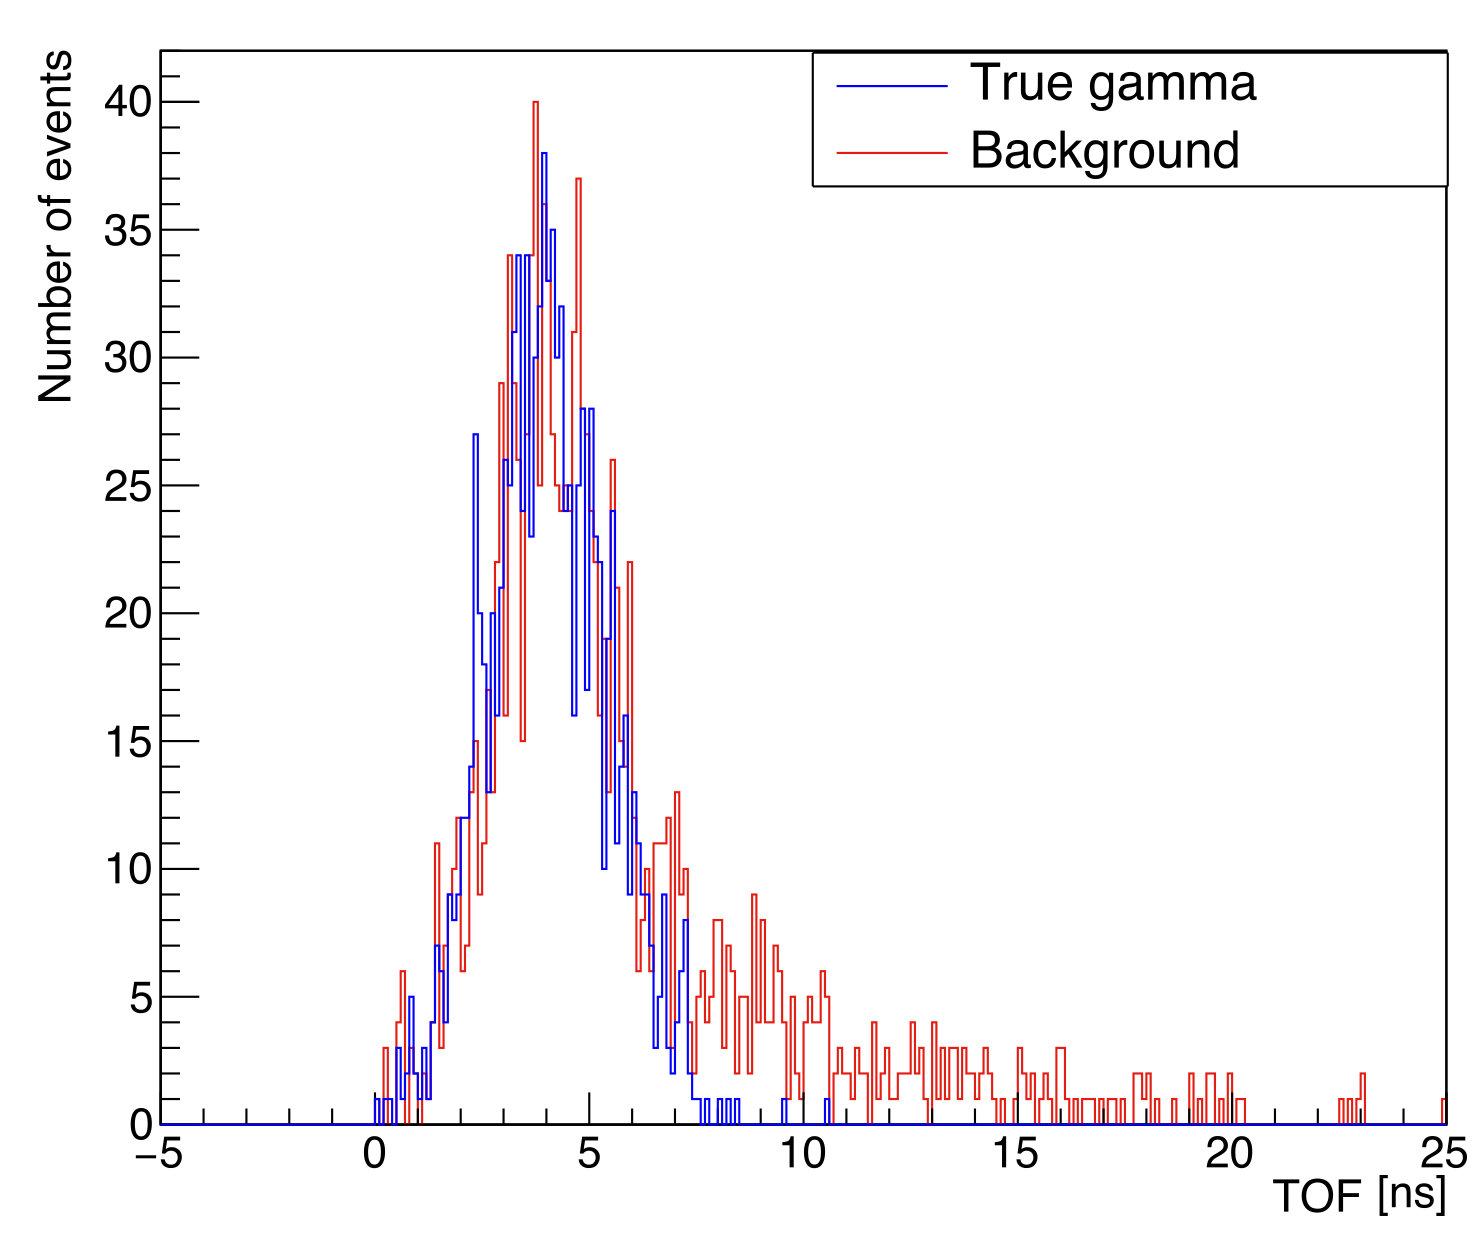
\includegraphics[width=0.6\textwidth]{03_GraphicFiles/chapter4_HTsimu/TOFspectrum.png}
  \caption{Time of flight spectra of true gamma coincidences (blue) and background events (red) obtained with $10^{8}$ 160~MeV independent incident protons.}	
  \label{chap4::fig::fig_TOF_distribution_CC_simulation_Hadronth}
\end{figure}

\item Energy selection: energy thresholds are defined for the event detection. 50~keV and 100~keV are set as lower threshold for the energy deposited in a single silicon layer and \gls{bgo} block, respectively. For a complete event, a total absorbed energy lower limit is set to 1~MeV. In addition to the effect of background rejection, this selection also reduces the impact of partially absorbed photons.

Further energy selections, assuming for instance $E_1+E_2$ equal to one of the strong gamma lines, have been applied by other authors~\parencite{Draeger2017}. Also, filters checking the possibility of reconstructing a Compton cone could be used. At this stage we did not consider such approaches in order to cope with simple considerations on signal to noise on raw data.

\end{itemize}

\subsection{Reconstruction algorithms}\label{chap4::subsec::MatMeth:reconstruction}
Once the coincidences are defined and selected according to the fixed physical cuts, the \gls{pg} emission point has to be reconstructed for each event. This can be done via analytic or iterative algorithms based on the Compton kinematics. Both are presented in the following sections.

\subsubsection{Line-cone algorithm}\label{chap4::subsubsec::line_cone}
The reconstruction via line-cone algorithm exploits the energy deposit and position information collected by the camera in addition to the beam spatial information provided by the hodoscope. Thanks to the deposited energies in the detectors and the interaction positions, a cone surface is analytically defined via the Compton equation~\ref{chap2::eq::ComptonAperture}. \figurename~\ref{chap4::fig::fig:reconstruction_scheme} shows a sketch of the reconstruction principle. The interaction position in the scatterer gives the cone apex and the line connecting the interaction positions in scatterer and absorber gives the cone axis. We assume that the initial energy of the gamma ray is fully absorbed in the absorber. This assumption has been investigated and the results are shown in section~\ref{chap4::subsec::Results_relefficiency}. In order to constrain the reconstruction, the beam direction is used to limit the possible solutions (lying on the reconstructed cone surface) to two points (intersection of the beam direction and the reconstructed cone). At this stage we do not consider the lateral beam spread in the target, due to multiple scattering. The set of all the reconstructed points gives the emission source distribution. The final image is the mono-dimensional projection of the prompt gamma emission profile. 

\begin{figure}
\centering
  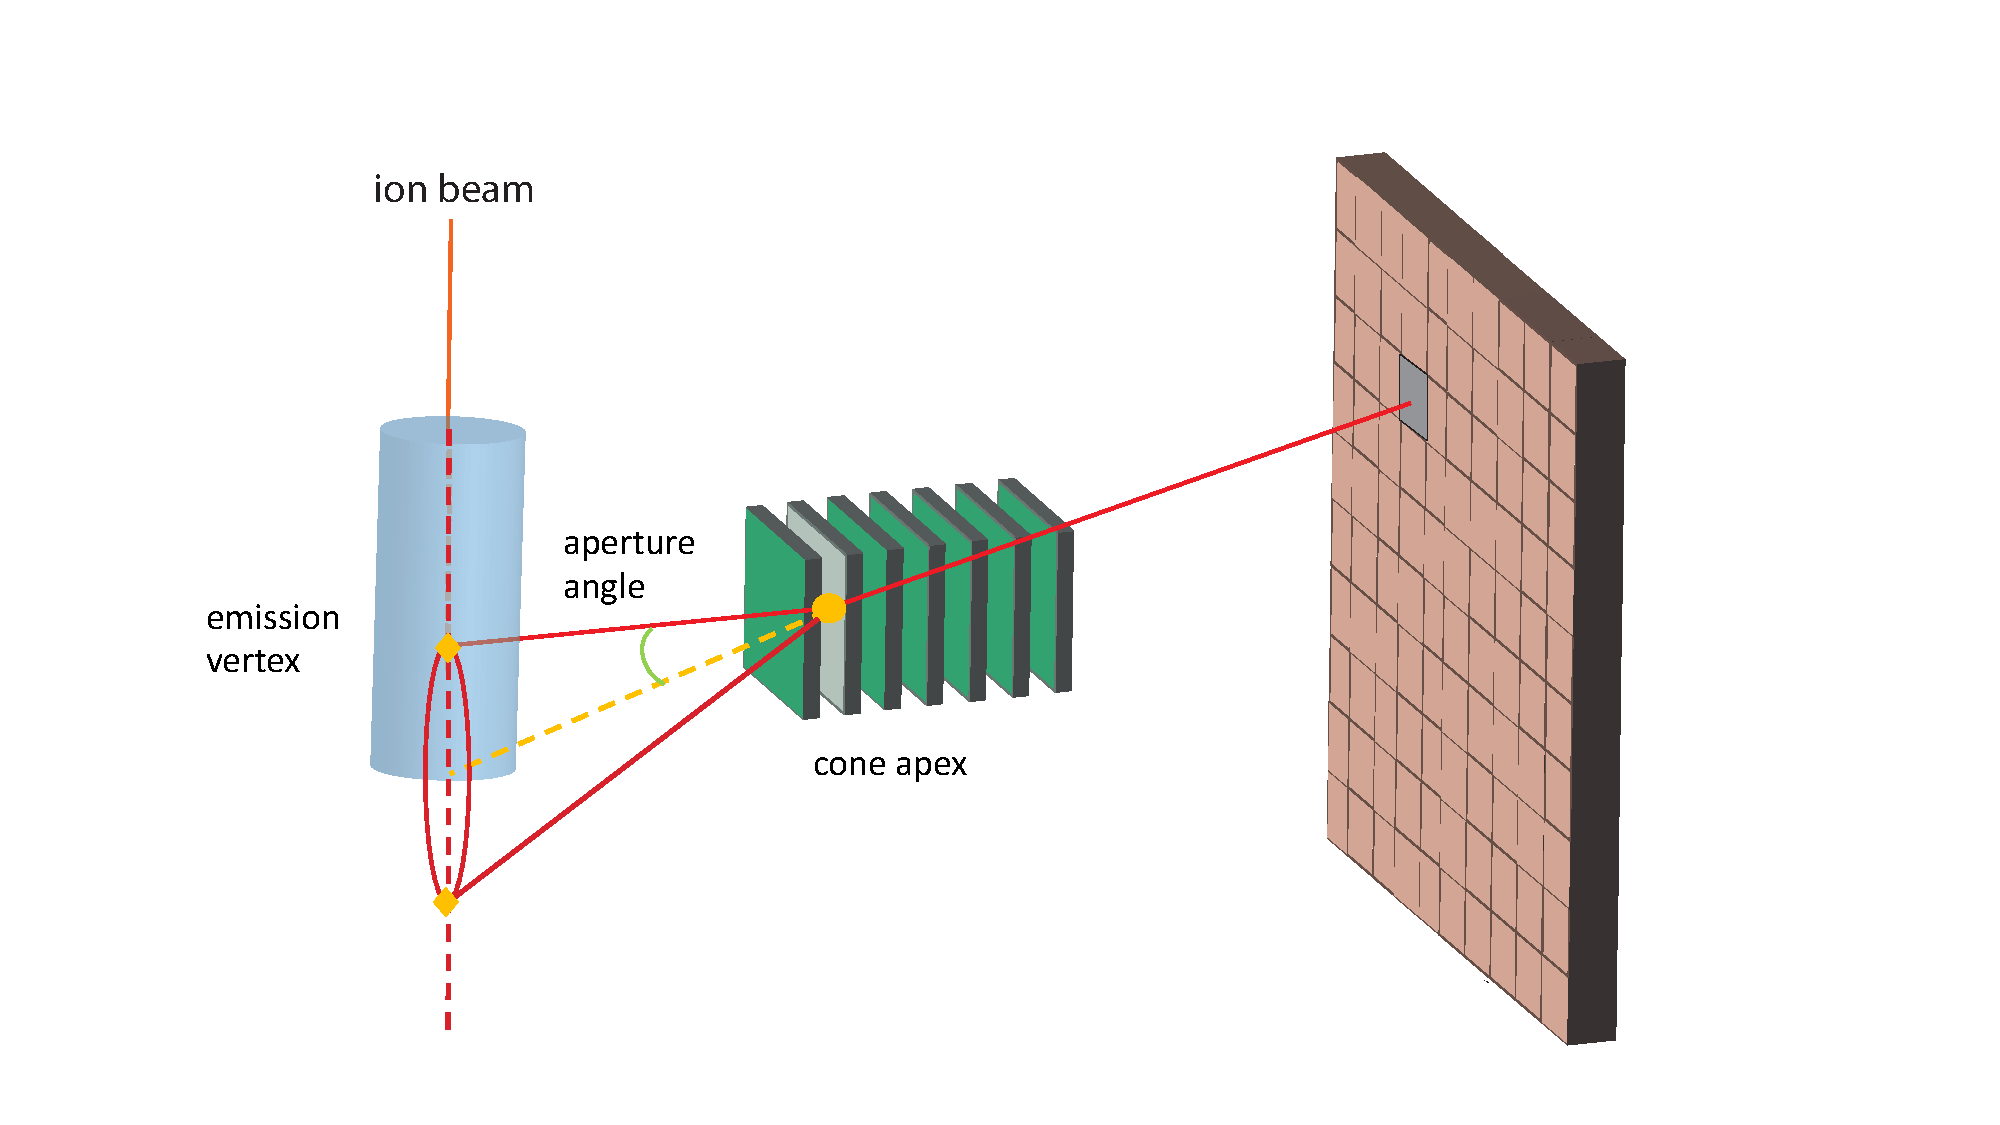
\includegraphics[width=0.8\textwidth]{03_GraphicFiles/chapter4_HTsimu/reconstruction_scheme}
  \caption{Scheme of the reconstruction principle for Compton events. For line-cone reconstruction methods, two points are extracted for each event (diamonds in the figure), provided by the intersection between the reconstructed Compton cone and the beam line. The reconstructed image is strictly mono-dimensional. For the iterative \gls{mlem} algorithm, each algorithm iteration adds constraints to the reconstructed cone surfaces, leading to  a three-dimensional image.}	
  \label{chap4::fig::fig:reconstruction_scheme}
\end{figure}

\subsubsection{LM-MLEM algorithm}\label{chap4::subsubsec::lmmlemalgo}	
The iterative methods allow to get a three-dimensional image reconstruction, potentially by taking into account the spatial resolution and the energy resolution of the detectors. Several iterative algorithms have been developed for Compton event reconstruction~\parencite{Schone2010, Zoglauer2011, Gillam2011, Mackin2012, Huang2018, Taya2017, Schone2017}.

The \gls{lm-mlem} algorithm is a MLEM version which enables one to reconstruct the image directly from the list of detected events.
The features of the \gls{lm-mlem} algorithm used for this study are detailed in~\cite{Hilaire2014}.

\subsection{Performance study}\label{chap4::subsec::MatMeth:performance}
In this section the parameters studied for the camera performance evaluation are explained. The study is mainly divided into four sections:
\begin{itemize}
\item Detection efficiency of various types of true coincidences: the camera efficiency for the detection of the various kinds of true coincidences defined in section~\ref{chap4::subsec::MatMeth::events} is studied by means of mono-energetic irradiation with point-like sources as a function of the incident gamma energy;
\item Absolute efficiency: the camera absolute efficiency for the detection of events with a single scatterer layer involved is studied by means of mono-energetic irradiation with point-like sources as a function of the incident gamma energy and the source position with respect to the camera;
\item Rate of background coincidences: with proton and carbon beams interacting with the \gls{pmma} phantom, the rate of background and true detected coincidences (for events with a single scatterer layer involved) is studied as a function of the beam intensity;
\item Camera precision: the camera capability of identifying the fall-off of the prompt-gamma emission profile is tested and the two reconstruction methods presented above are compared (for events with a single scatterer layer involved). 
\end{itemize}

\subsubsection{Detection efficiency of various types of true coincidences}\label{chap4::subsubsec::relEff}
The efficiency is crucial for the Compton camera performances and for its possible application in treatment monitoring. An efficient monitoring system should be ideally in real time, in order to allow for a treatment adaptation or interruption in case of severe issues detected in the delivered dose profile with respect to the planned treatment. In order to achieve an online detection of such deviations, given the limited prompt gamma emission rate per incident ion~\parencite{Ortega2015}, a high detection efficiency is required to perform a monitoring on, ideally, a beam spot basis. In addition to this, the absolute detection efficiency directly affects the image reconstruction quality, which is in general increased for increased statistics.

The efficiency in the detection of specific kinds of events detailed in section~\ref{chap4::subsec::MatMeth::events} has been studied with the irradiation from point-like mono-energetic gamma sources. The setup is the same as \figurename~\ref{chap4::fig::fig_setup_CC_simulation_Hadronth}, with the exception of the PMMA phantom which is removed to leave the gamma source in air. Different energies have been tested to mimic different prompt gamma lines: 300~keV, 500~keV, 1~MeV, 2~MeV, 4~MeV, 6~MeV. No time structure is reproduced for this part of the study.
In addition, the rate of events with an almost full primary energy absorption has been studied for the various kinds of coincidences as a function of the primary gamma energy. The threshold for the energy absorption has been set to 90\% of the primary gamma energy. 
The results of this preliminary study (see section~\ref{chap4::subsec::Results_relefficiency}) determined the choice to limit the next investigations to events with a single scatterer plane involved; all events with more than one scatterer layer hit have been rejected for the analysis described from section~\ref{chap4::subsubsec::absEff} and the results presented from section~\ref{chap4::subsec::Results_efficiency}.

\subsubsection{Absolute detection efficiency}\label{chap4::subsubsec::absEff}

The absolute efficiency $\epsilon$ for the detection of coincidences with a single scatterer plane hit is defined as:
\begin{equation}
\epsilon =\frac{\mathrm{N}\gamma_{\mathrm{coinc}}}{\mathrm{N}\gamma_{\mathrm{total}}},
\end{equation}
\label{chap4::eq::equation_absEff}
with $N\gamma_{\mathrm{coinc}}$ the number of gamma events corresponding to the selected true coincidences, $N\gamma_{\mathrm{total}}$ the total number of emitted gammas.

In addition to its dependence on the gamma energy in the range 300~keV - 6~MeV (see section~\ref{chap4::subsubsec::relEff}), the absolute efficiency has been also studied as a function of the point-like source position. The source is set in the range $-300$~mm to $+300$~mm (with the center of the camera transverse section set in the position 0), and moved with variable length steps, up to 1~cm. The movement followed the transverse axis of the camera. 

\subsubsection{Rate of random coincidences}\label{chap4::subsubsec::random}

As the Compton detection principle relies on time coincidences, in addition to the main importance played by the detectors energy resolutions, the beam intensity and time structure are important parameters to be studied in order to assess the possible clinical implementation of a Compton detection based monitoring of ion beam treatment. The ability of the detection system to distinguish between true and random coincidences, i.e.~the resulting signal over noise ratio, strongly depends on the beam time structure. The number of true and background coincidences is studied as a function of the beam intensity, before and after data reconstruction via line-cone algorithm~(see section~\ref{chap4::subsec::MatMeth:reconstruction}). To be noticed that, following the results of the efficiency study (see section~\ref{chap4::subsec::Results_relefficiency}), only events with one single scatterer layer hit are selected. 

The range of intensities is defined in order to cover a wide range of operation: from a very low beam intensity to a realistic clinical particle rate. Therefore, for proton and carbon ions, the lowest beam intensity is set to 0.1 particles per bunch on average, while the upper limit is set to 217 protons or 70 carbon ions per bunch. All the simulations are performed with a total of $10^{8}$ primary protons and  $2\times10^{5}$ primary carbon ions (see section~\ref{chap4::subsubsec::beam_modeling}). For the analysis of the results, the coincidence yields are scaled to the number of incident ions and the beam intensity to the average number of ions per bunch.

\subsubsection{Camera precision}\label{chap4::subsubsec::MatMeth:precision}

The camera precision is defined as the difference between the predicted \gls{pg} \gls{fop} (according to the treatment planning) and the detected one.
In this study, a reference profile has been defined as the reconstructed emission vertex profile at high statistics ($\mathrm{10^{10}}$ incident protons). This \gls{fop} is used as reference and compared to the ones at lower statistics, deduced as described in the following.

For the \gls{lm-mlem} reconstruction, the reconstruction volume is set to $20\times40\times1$~cm$^3$ around the expected \gls{fop}, with a $101\times201\times5$ voxel matrix. To be noticed that the two reconstruction methods produce different results: the line-cone method is based on the beam direction information, so that it naturally returns a mono-dimensional image as result, while the \gls{lm-mlem} method is able to reconstruct the \gls{pg} emission distribution in three dimensions. A mono-dimensional projection along the beam direction is used for the fall-off identification and for a direct comparison of the line-cone method.
The \textit{SmoothKern} method, with the Nadaraya-Watson regression~\parencite{Nadaraya1964, Watson1964}, is used to smooth the reference profiles in order to reduce relative statistical fluctuations.

A \gls{roi} ranging from $y=0$ mm to $y=+100$ mm is defined around the expected \gls{fop}, located at $y=+50$~mm in the phantom. The reference reconstructed profiles are modeled in the \gls{roi} by a linear combination of \gls{nurbs}~\parencite{Rogers2001}. 

The reference data set is normalized in order to obtain lower statistics profiles, in the range 1$\times$10$^8$ to 5$\times$10$^9$. Statistical fluctuations, randomly extracted following a Poisson law, are added to the obtained \gls{pg} profiles to mimic realistic reconstructed profiles. This method is used to reduce the analysis time.

For each chosen statistics, 1000 \gls{pg} profiles are generated and a custom minimization method is applied to deduce the minimal shift between the reference profile and the one at lower statistics. The minimization algorithm shifts the reference profile in a 60~mm range, between $-30$~mm and $+30$~mm with respect to the initial position, with a step of $0.1$~mm, and for each position it compares its position to the low statistics profile by calculating the $\chi^2$ as follows:
\begin{eqnarray}
\chi^2 = \sum\limits_{i=1}^{N_{bin}} {(y_{\mathrm{sample,i}}-y_{\mathrm{NURBS,i}})^2},
\end{eqnarray}
where for every bin $i$ $y_{\mathrm{sample}}$ is the number of events in the low statistics profile, $y_{\mathrm{NURBS}}$ is the number of events for the reference profile \gls{nurbs} (scaled at the same low statistic). 
The described approach is robust and allows to avoid artifacts at low statistics.
The global minimum of all the calculated $\chi^2$ is then retrieved and the shift associated to this value is added to the shift distributions. 
The standard deviation of the distribution resulting of the thousand results gives the precision of the camera for a given number of incident protons. 

\section{Results}\label{chap4::sec::results}

The possible implementation of the CLaRyS Compton camera as a monitoring system for ion beam therapy has been investigated. The camera has been exposed to point-like gamma sources to study the detection efficiency.
A \gls{pmma} cylindrical phantom has been simulated and exposed to proton and carbon beams at increasing intensities for an analysis of the prompt gamma detection environment (background, random coincidence contamination). The camera precision in the identification of the fall-off of the prompt gamma emission profile has been investigated.
In the following sections we show the obtained results.  

\subsection{Detection efficiency of various types of true coincidences}\label{chap4::subsec::Results_relefficiency}
\figurename~\ref{chap4::fig::eff_evKind} shows the Compton camera efficiency in detecting the kinds of coincidence events described in section~\ref{chap4::subsec::MatMeth::events}, as a function of the gamma energy in the prompt-gamma energy range (between 300~keV and 6~MeV). The results show how the single events, consisting in the coincidence between an energy deposit in a single scatterer layer and in one single absorber block, decreases at increasing energy, in favor of an increase in the number of electron escape events (consisting in one primary photon Compton interaction in one scatterer layer, at least one interaction of the Compton escaped recoil electron in a different scatterer layer, and one primary photon interaction in one single absorber block). At the maximum investigated primary gamma energy,  the amount of electron escape collected events is more than 35\%. However, the single events represent more than 60\% of the total amount of collected events in all the explored energy range, so that the results in the following paragraphs are focused on this kind of events (with the other kinds of events rejected at the analysis stage), as first approach for a feasibility study. The amount of 3 or more photon-interaction events is limited and negligible over the whole energy range.

\begin{figure} [!hbtp]	
\centering
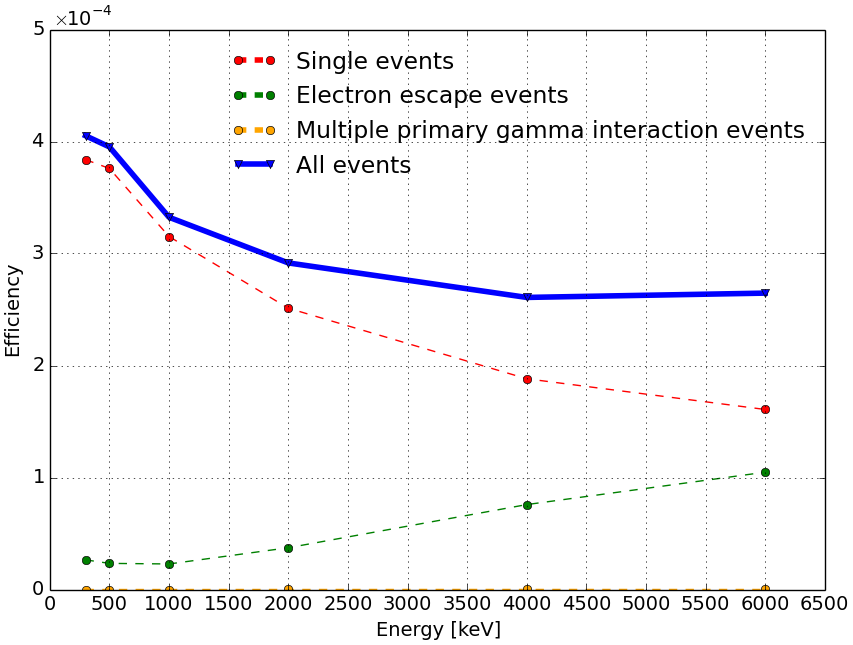
\includegraphics[width=0.6\textwidth]{03_GraphicFiles/chapter4_HTsimu/new/effVSenergy_trigger.png}
\caption{Compton camera efficiency as a function of the gamma energy for the different kind of possible coincidence events (see section~\ref{chap4::subsec::MatMeth::events}), as a function of the gamma energy.}
\label{chap4::fig::eff_evKind}
\end{figure}

\begin{figure} [!hbtp]	
\centering
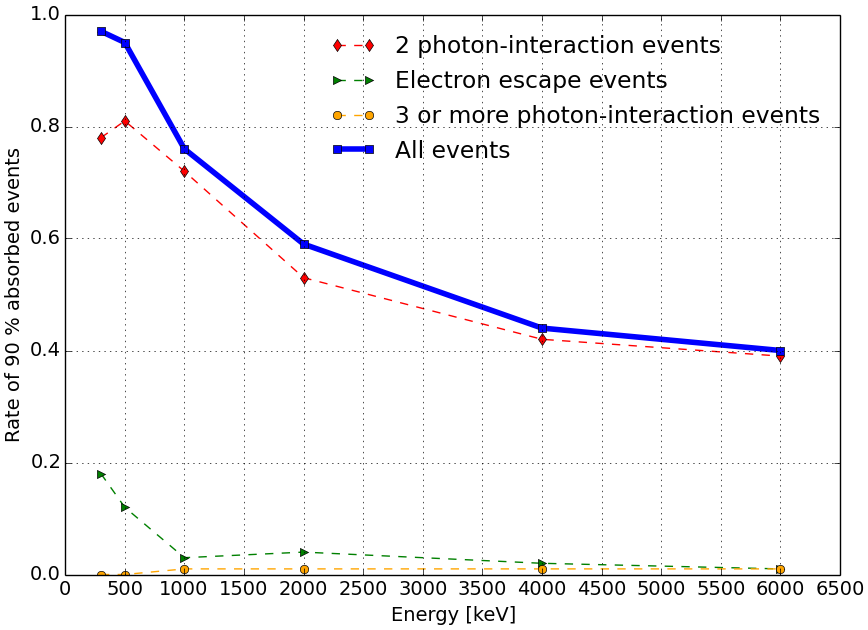
\includegraphics[width=0.6\textwidth]{03_GraphicFiles/chapter4_HTsimu/new/90absFracVSenergy_hadronth.png}
\caption{Ratio between coincidence events with more than 90\% of the primary photon energy absorbed in the detector layer and all detected coincidences as a function of the gamma energy. The curves shown the results for the different kind of possible coincidence events and for the all collected coincidences.}
\label{chap4::fig::rate_full_abs}
\end{figure}

\figurename~\ref{chap4::fig::rate_full_abs} shows the rate of events with more than 90\% of the primary gamma energy deposited in the detector layers. The rate of 90\% absorbed events is reported for the different kinds of detected coincidences. As expected, the rate of almost fully absorbed events decreases as the energy increases, in a range between more than 80\% and 40\% for 300~keV and 6~MeV primary photon energy, respectively. The most of the 90\% absorbed events are single events, with the electron escape and multiple ones negligible for primary gamma energies above 1~MeV. At lower energy, the Compton recoil electron is often able to exit the scatterer layer where the Compton interaction takes place, but can be lost without further interactions, so that this kind of events is considered as single with an energy absorption below 90\%. This can explain the decrease of single almost full absorption at 300~keV. If the electron interacts with a scatterer layer, it is generally absorbed at low energy, explaining the increasing electron escape absorbed events below 1~MeV. 
As mentioned, these results led to the choice of limiting the further analysis (from section~\ref{chap4::subsec::Results_efficiency}) to events with a single scatterer layer involved, as first approach.

 \subsection{Absolute detection efficiency}\label{chap4::subsec::Results_efficiency}
\figurename~\ref{chap4::fig::efficiency_study} shows the absolute gamma detection efficiency as a function of the gamma source position with respect to the center of the camera in the transverse plane. On the left side, we show the results achieved with an ideal detector (i.e. without energy detection threshold). On the right side realistic energy thresholds (50~keV for the scatterer layers and 100~keV for the absorber) are applied on each detector section.

\begin{figure} [!hbtp]	
\begin{subfigure}[b]{.5\textwidth}
\centering
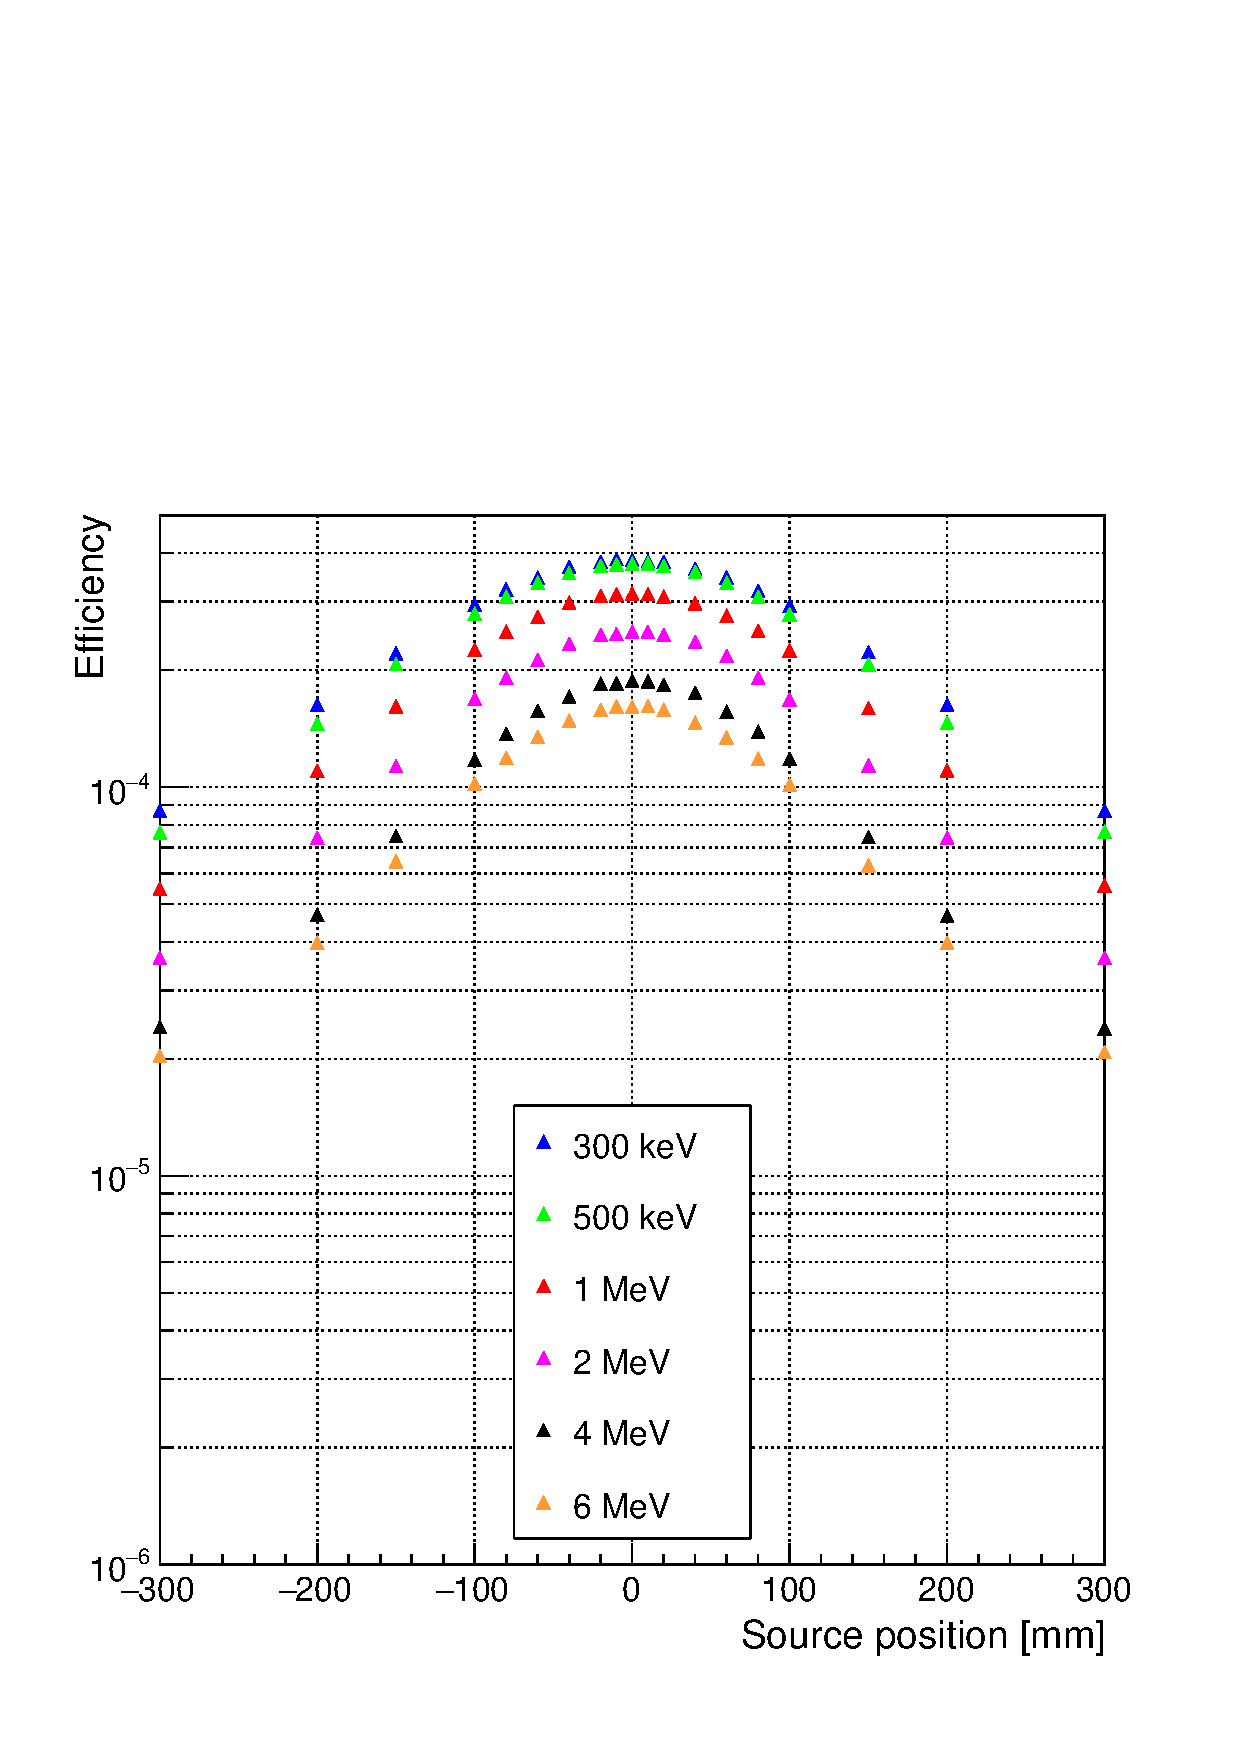
\includegraphics[width=0.9\textwidth]{03_GraphicFiles/chapter4_HTsimu/new/EffVSpos_noCut_simple.pdf}
\caption{}
\label{chap4::fig::effPos_noCut}
\end{subfigure}
\begin{subfigure}[b]{.5\textwidth}
\centering
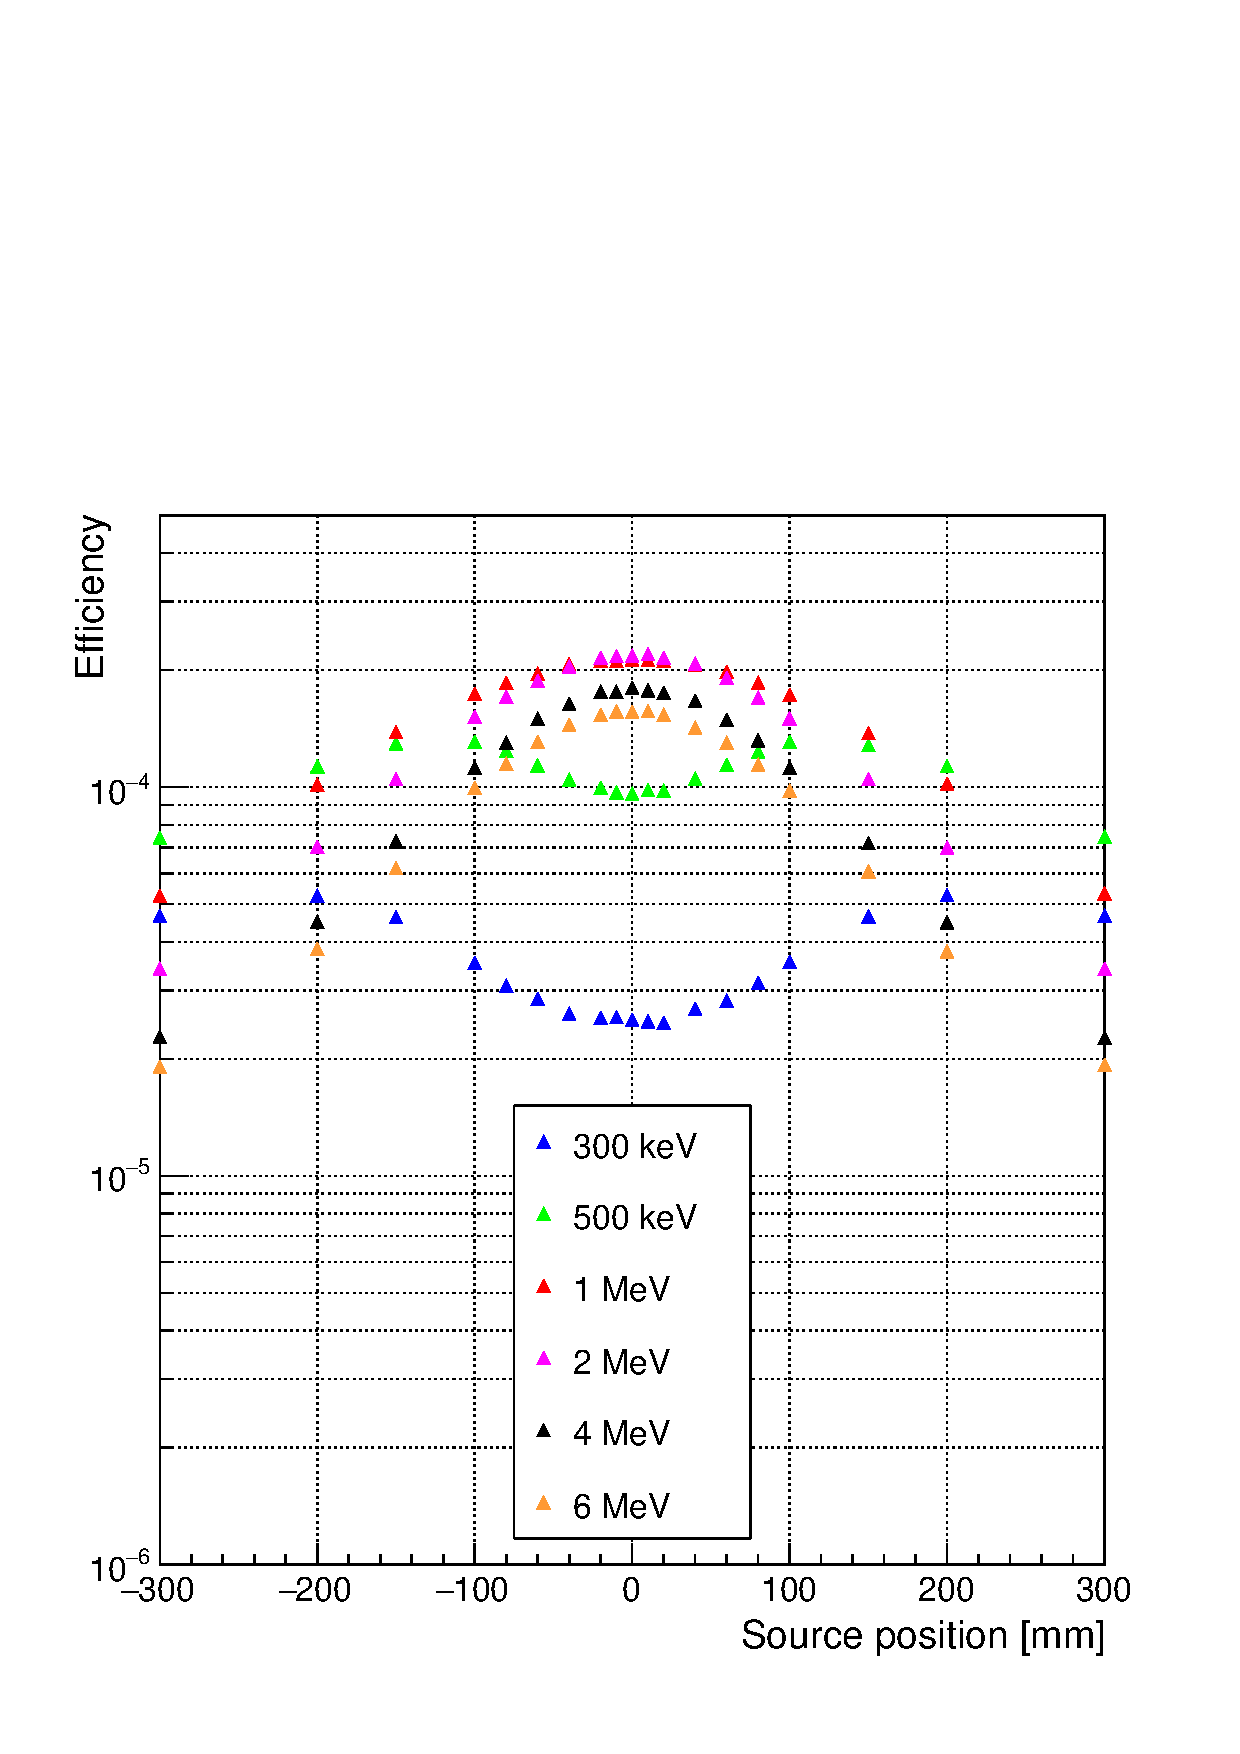
\includegraphics[width=0.9\textwidth]{03_GraphicFiles/chapter4_HTsimu/new/EffVSpos_CutSingle_simple.pdf}
\caption{}
\label{chap4::fig::effPos_Cut}
\end{subfigure}
\caption{Absolute Compton camera efficiency as a function of the gamma source position for different gamma energies, in the range between 300~keV to 6~MeV. The left side shows the camera efficiency with no detection energy threshold. In the right side, detection energy thresholds are applied to reproduce a realistic scenario (lower limit of 50~keV for the scatterer, 100~keV for the absorber). These values can change for the final configuration, according to the detector energy resolutions achieved.}
\label{chap4::fig::efficiency_study}
\end{figure}

As expected according to the interaction probability energy dependency, the efficiency is higher for low gamma energies, and it lies in the range $4\times10^{-4}$ at 300~keV and $1.5\times10^{-4}$ at 6~MeV at the center of the camera. Moreover, it can be noticed how the efficiency slightly drops as the point source is shifted away from the camera center: efficiency reductions at 500~keV and 4~MeV are respectively of 25\% and 35\% with the source at 300~mm distance from the camera center, with respect to the value detected in central position. This effect is more important for high energies, for which the incident gamma is less deflected in the scatterer for the same energy deposited compared to a low energy gamma.\\  
\figurename~\ref{chap4::fig::effPos_Cut} shows the effect of realistic camera detection thresholds as opposed to ideal detection. The gamma detection efficiency drops of a factor ranging from about 1.25 to more than an order of magnitude for the central detection area for energies in the range 300~keV to 2~MeV respectively. The effect is reduced by the distance of the source from the center of the camera. Negligible effects are detected for positions with a distance greater than 200~mm from the center of the camera, and for any distance at energies above 2~MeV, while the efficiency is reduced in the central area of the camera for energies below 4~MeV.\\
 
\subsection{Rate of background coincidences}
\label{chap4::subsec::Results_beamInt}
 
In \figurename~\ref{chap4::fig::coincidences}, the different components of the signal resulting from the \gls{pmma} exposure to proton and carbon ion beams are shown as a function of the beam intensity. The true coincidences represent scatterer-absorber time coincidences generated by the same gamma ray (only single events). All the other coincidence types compose the background. The collected data sets are reported with and without the applied time-of-flight discrimination, mainly employed for neutron rejection, as mentioned in section~\ref{chap4::subsec::MatMeth::TOF_Ecut}.


\begin{figure} [!h]
\begin{subfigure}[b]{.5\textwidth}
\centering
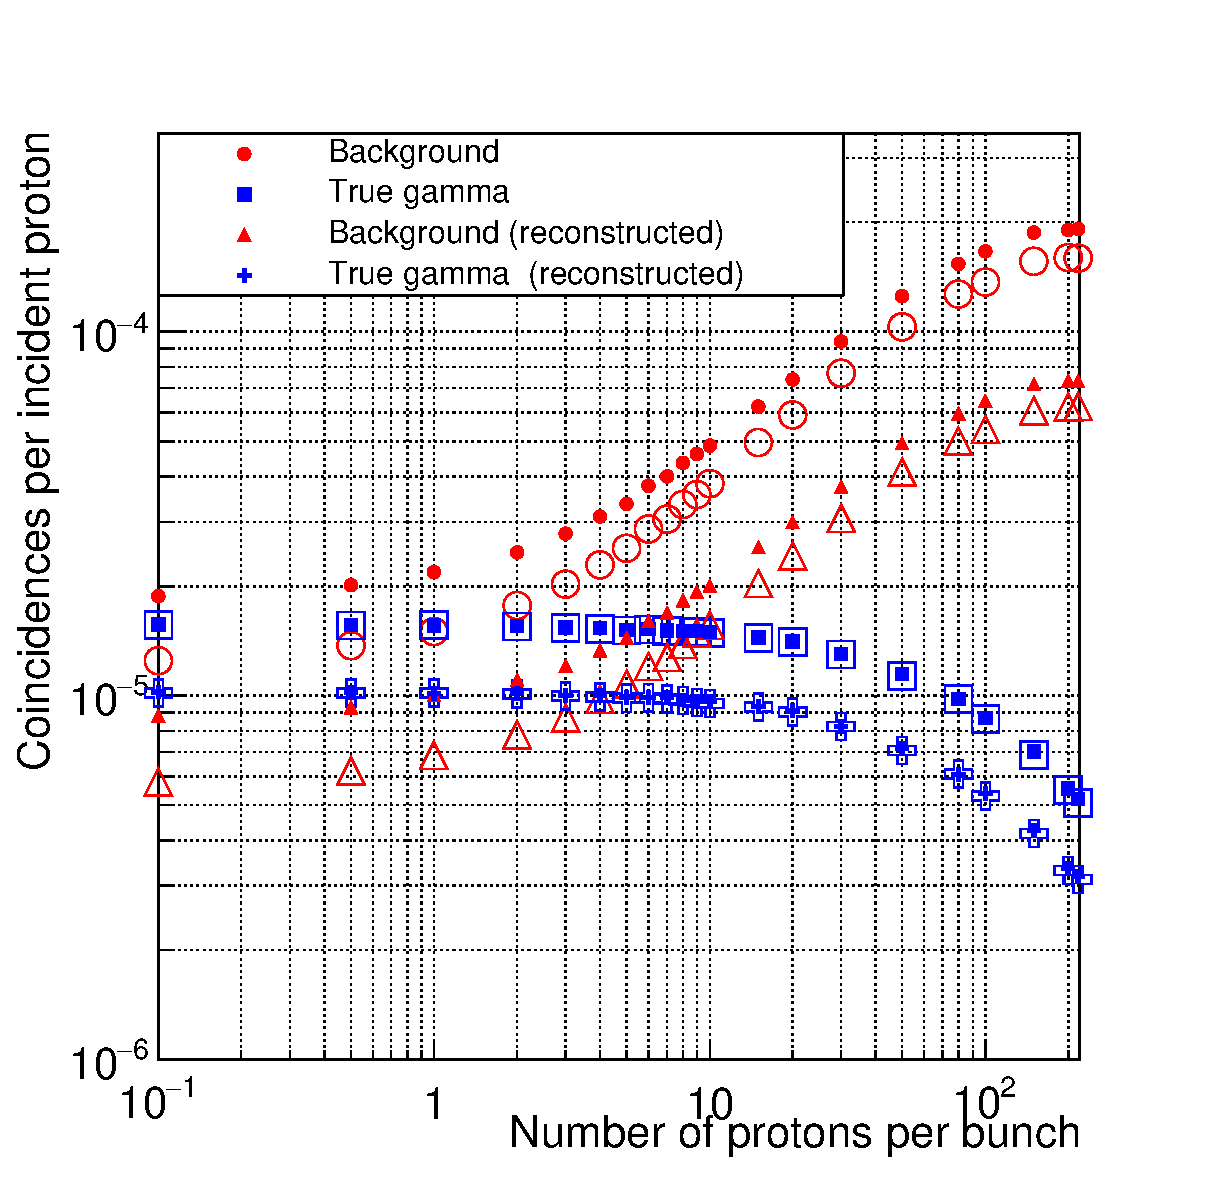
\includegraphics[width=0.9\textwidth]{03_GraphicFiles/chapter4_HTsimu/new/coincYields_protons.eps}
\caption{}
\label{chap4::fig::coincYields_p}
\end{subfigure}
\begin{subfigure}[b]{.5\textwidth}
\centering
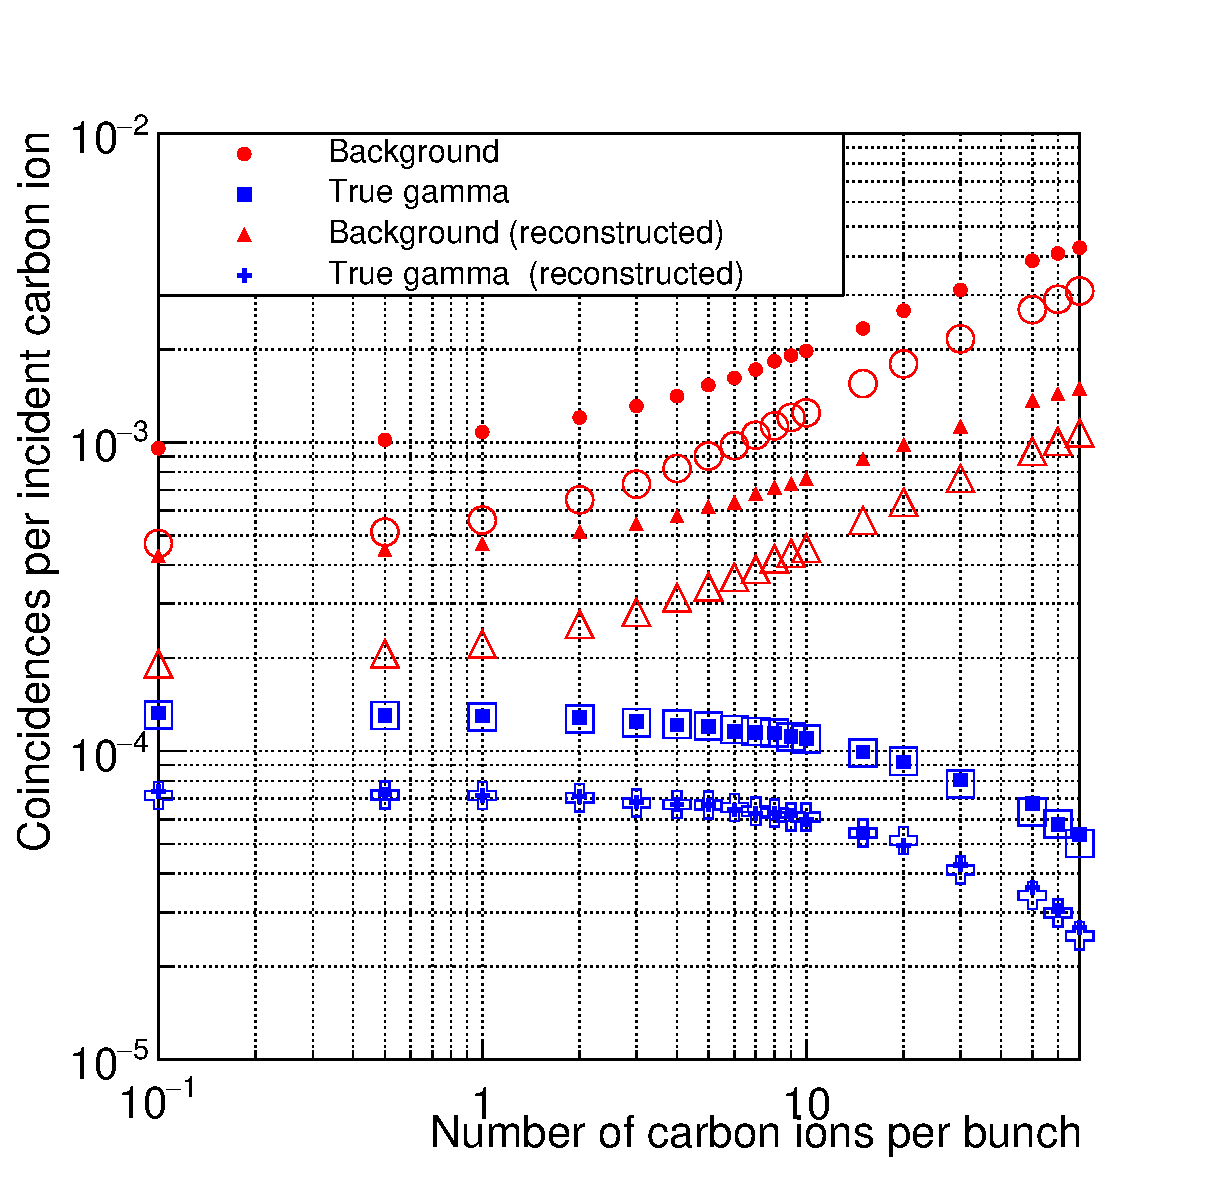
\includegraphics[width=0.9\textwidth]{03_GraphicFiles/chapter4_HTsimu/new/coincYields_Cions.eps}
\caption{}
\label{chap4::fig::coincYields_C}
\end{subfigure}
  \caption{Coincidences yield for protons (left) and carbon ions (right) as a function of the beam intensity. The intensity is reported as number of incident particles per bunch. The filled markers correspond to the collected data without time-of-flight discrimination, while this cut is applied to the data reported with empty markers. Moreover, the yields are given before and after the profile reconstruction with the line-cone algorithm.}
\label{chap4::fig::coincidences}
\end{figure}

In \figurename~\ref{chap4::fig::coincidences}(a) and (b) the amount of true gamma coincidences and background events are reported before and after reconstruction via line-cone algorithm as a function of the beam intensity for proton (a) and carbon ion (b) beams. In addition to this, for each curve realized with the complete collected data set, the related one obtained after time-of-flight selection of events is sketched (empty symbols). All the curves have been normalized to the number of incident ions.

The amount of background events (mainly random coincidences) increases with the increasing beam intensity: a factor of about 30 with respect to true gamma events is obtained for proton beams at  the intensity of 200 protons per bunch with no event selection, while a factor more than two times higher is reported for carbon ions in the same conditions. The \gls{tof} selection can slightly improve the \gls{snr} by reducing the amount of background events. The amount of true gamma events and background events becomes similar at the intensity of about 1 proton per bunch. As expected by the observation of \figurename~\ref{chap4::fig::fig_TOF_distribution_CC_simulation_Hadronth}, for intensity values below 1 proton per bunch, the ration between true and background events remains stable. 


\subsection{Camera precision}\label{chap4::subsec::Res_precision_reconstruction}
The camera precision in the fall-off identification is investigated with proton beams.
A data set corresponding to the irradiation of the \gls{pmma} phantom with a mono-energetic 160~MeV proton beam spot (10$^8$ protons) has been collected and analyzed with a clinical intensity of 200 protons per bunch and 1 proton per bunch on average. 
\figurename~\ref{chap4::fig::comparison} shows the results of the line-cone and \gls{lm-mlem} reconstructions of the simulated data for the two beam time structures applied at the analysis stage.  

\begin{figure}
\begin{subfigure}[b]{.5\textwidth}
\centering
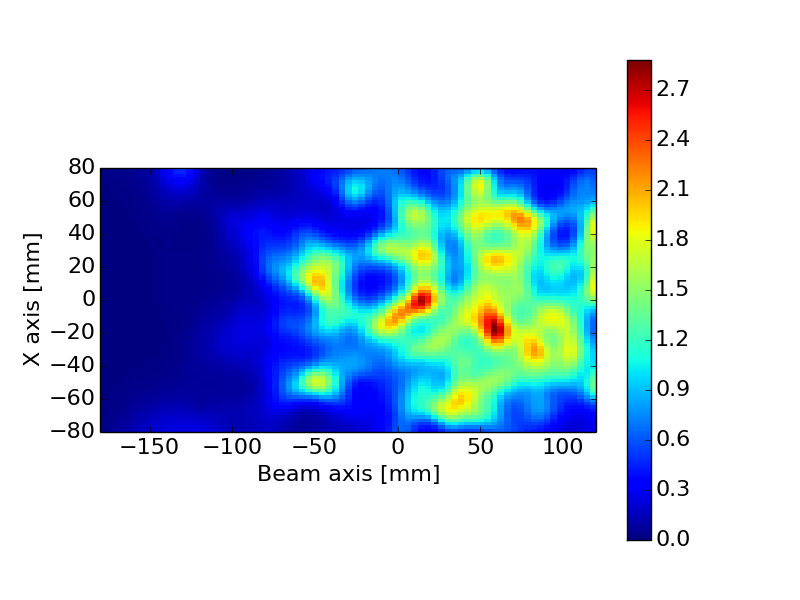
\includegraphics[width=0.9\textwidth,clip=true,trim=0 70 130 90]{03_GraphicFiles/chapter4_HTsimu/new/recon_200pBunch/projection2D_Z_corr_r20.png}
\caption{}
\label{chap4::fig::2Drecon_MLEM_200p}
\end{subfigure}
\begin{subfigure}[b]{.5\textwidth}
\centering
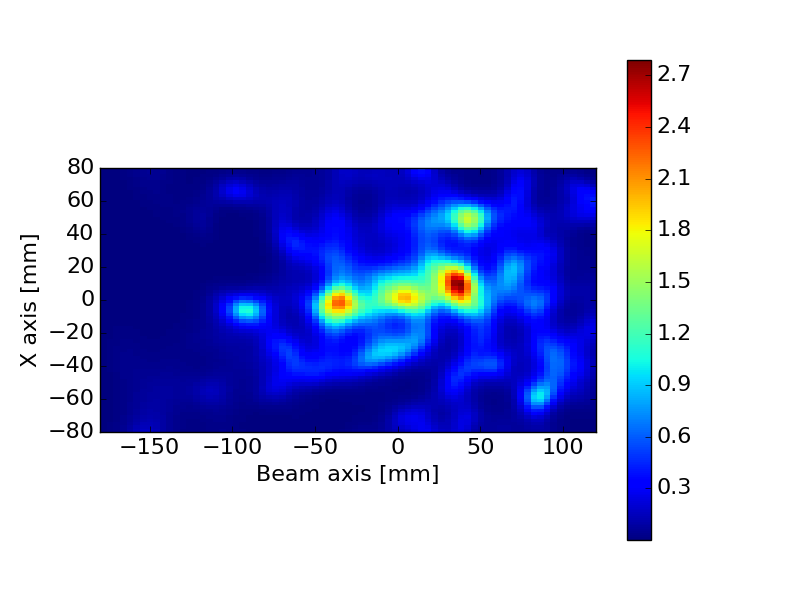
\includegraphics[width=0.9\textwidth,clip=true,trim=0 70 130 90]{03_GraphicFiles/chapter4_HTsimu/projection2D_Z_corr_r20.png}
\caption{}
\label{chap4::fig::2Drecon_MLEM_1p}
\end{subfigure}
\begin{subfigure}[b]{.5\textwidth}
\centering
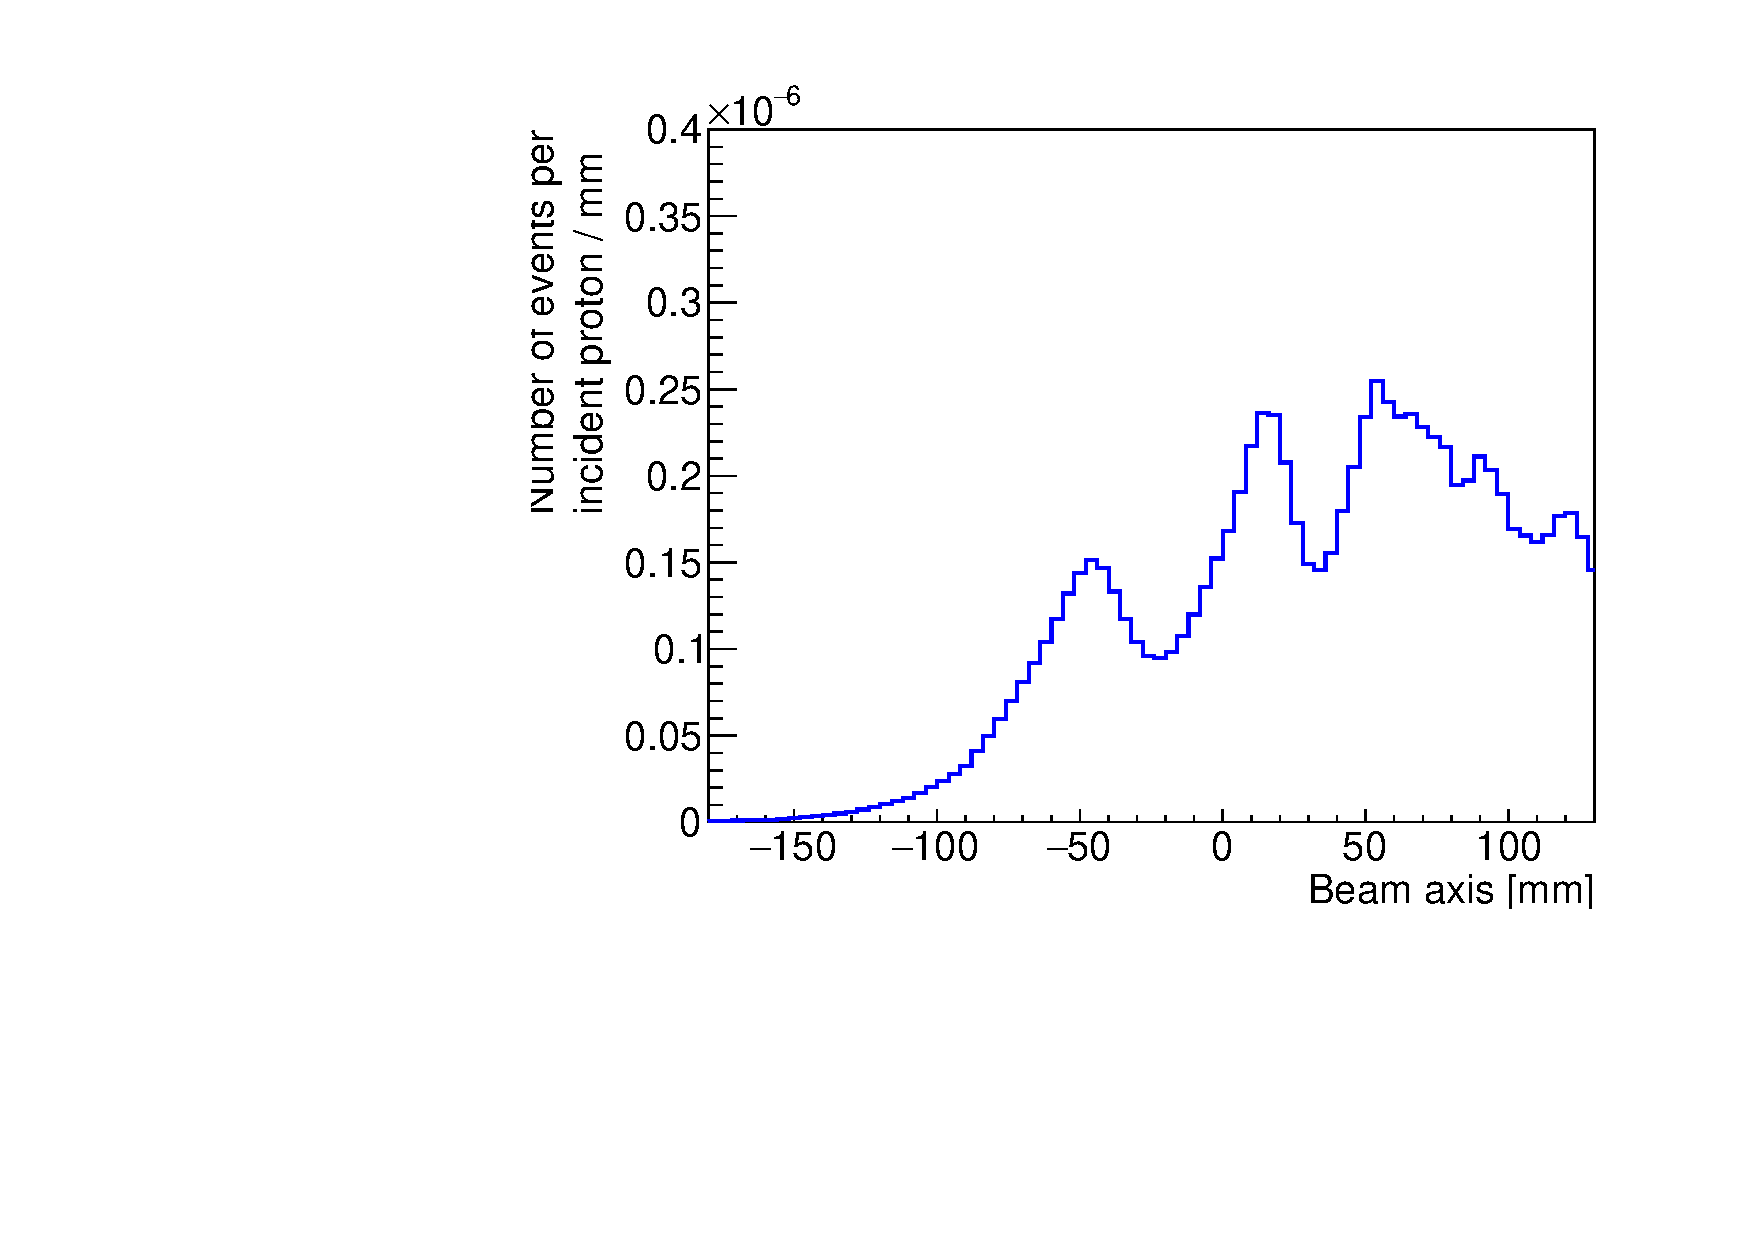
\includegraphics[width=0.9\textwidth]{03_GraphicFiles/chapter4_HTsimu/new/profile_MLEM_200pBunch.pdf}
\caption{}
\label{chap4::fig::1Drecon_MLEM_200p}
\end{subfigure}
\begin{subfigure}[b]{.5\textwidth}
\centering
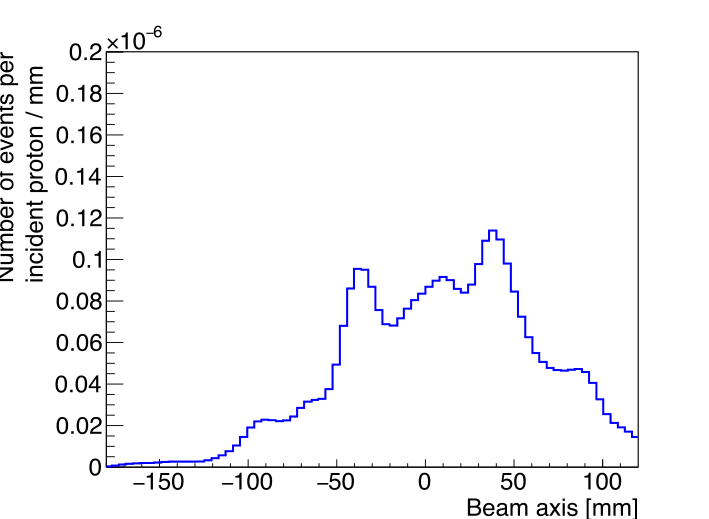
\includegraphics[width=0.9\textwidth]{03_GraphicFiles/chapter4_HTsimu/new/reconstructed_lowStat_profile_norm_mod.png}
\caption{}
\label{chap4::fig::1Drecon_MLEM_1p}
\end{subfigure}
\begin{subfigure}[b]{.5\textwidth}
\centering
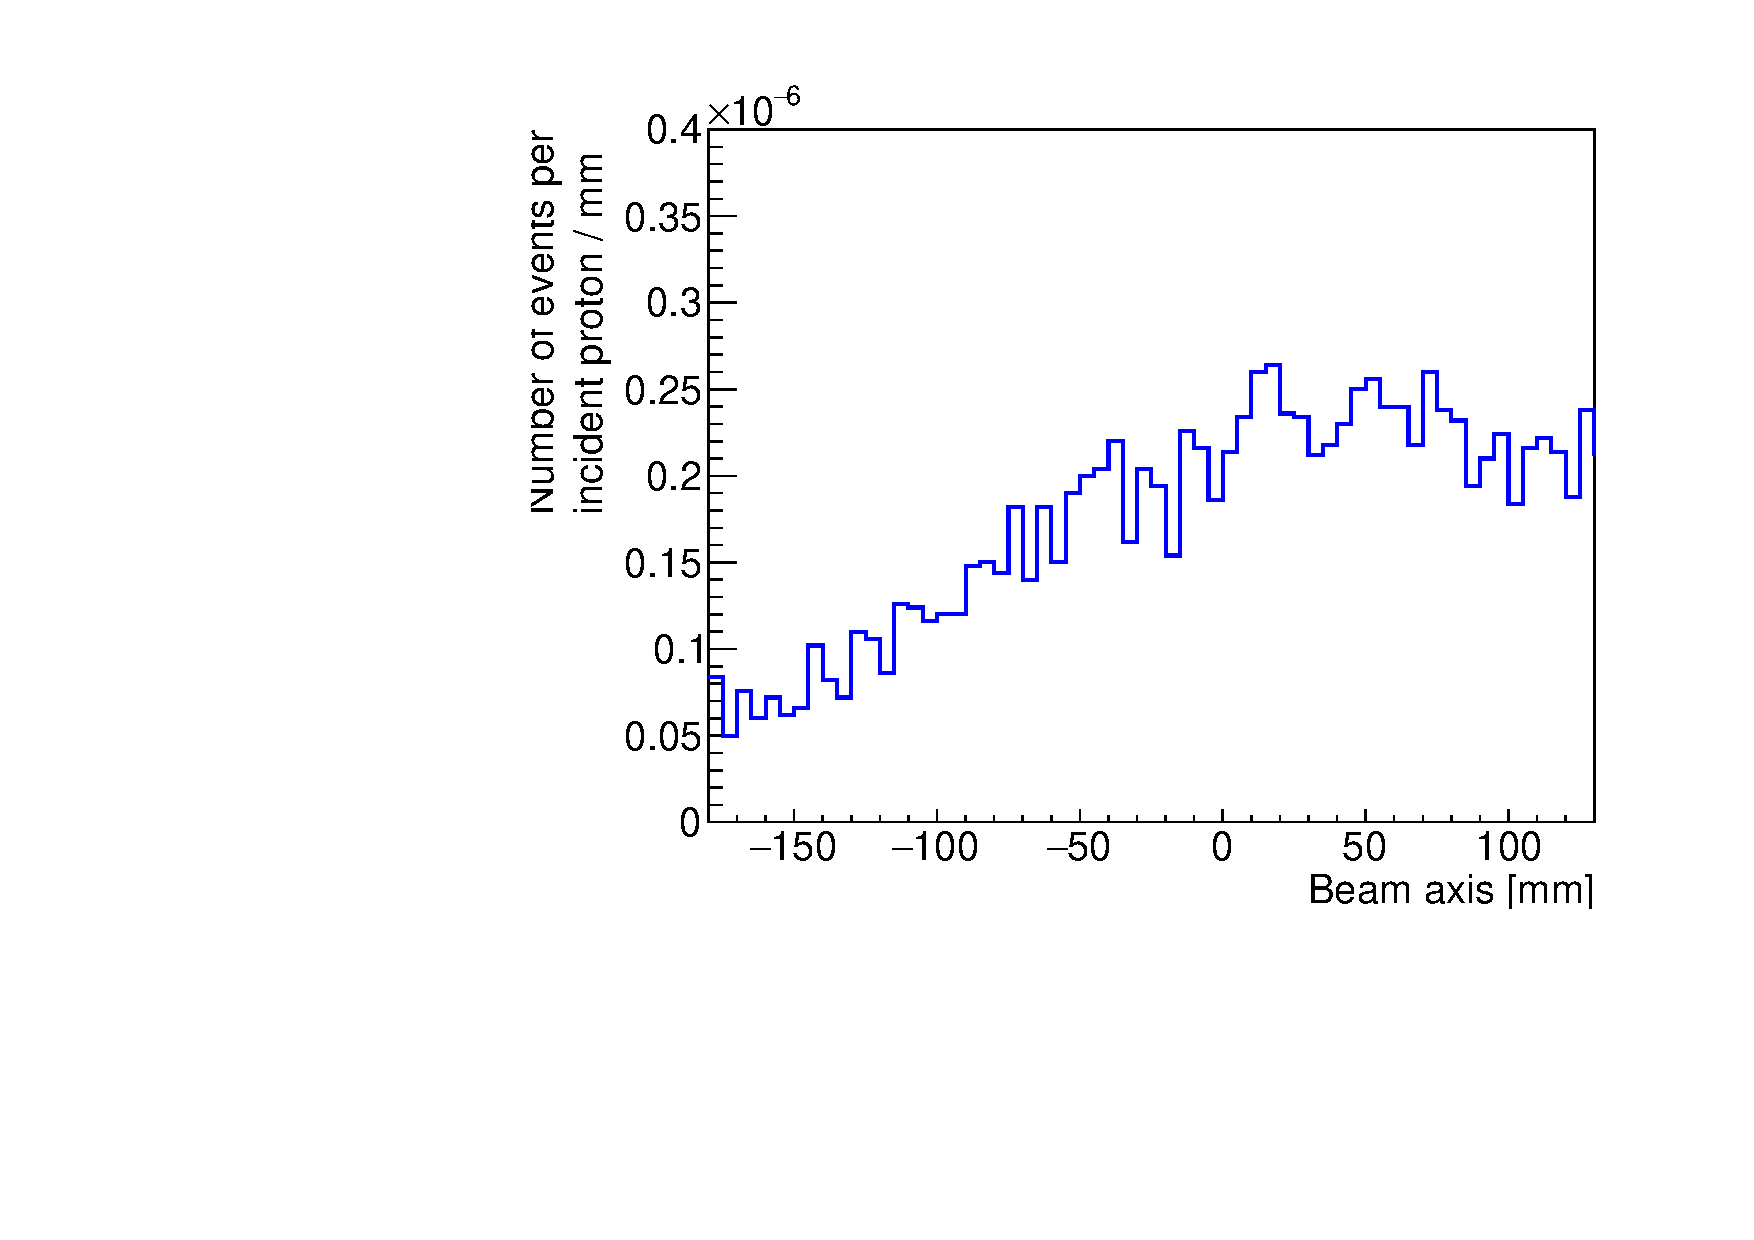
\includegraphics[width=0.9\textwidth]{03_GraphicFiles/chapter4_HTsimu/new/profile_lineCone_200pBunch.pdf}
\caption{}
\label{chap4::fig::1Drecon_LC_200p}
\end{subfigure}
\begin{subfigure}[b]{.5\textwidth}
\centering
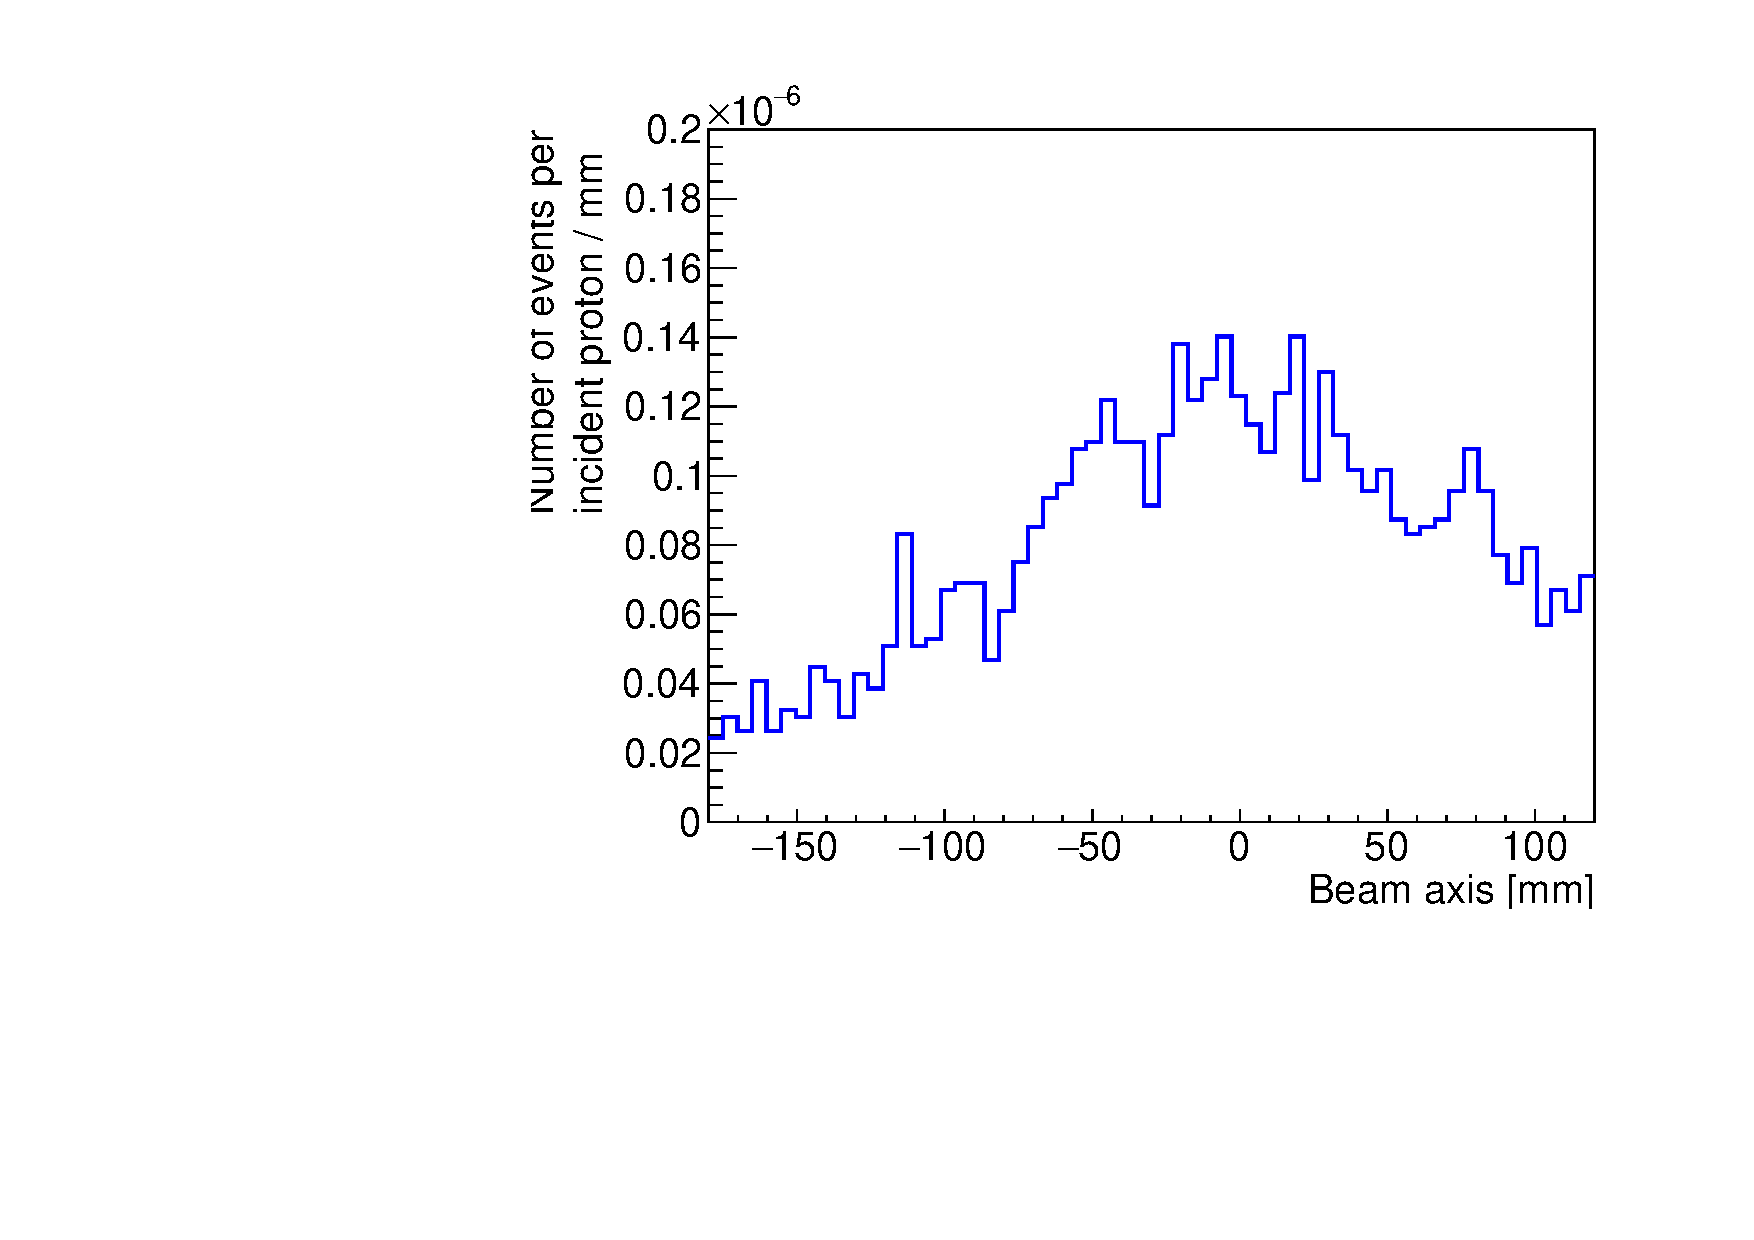
\includegraphics[width=0.9\textwidth]{03_GraphicFiles/chapter4_HTsimu/new/recon_profile_line-cone_lowStat_norm.pdf}
\caption{}
\label{chap4::fig::1Drecon_LC_200p}
\end{subfigure}
\caption{Line-cone and \gls{lm-mlem} reconstruction for a 160~MeV proton beam, $10^{8}$ total incident protons. In the left column, the beam intensity is 200 proton per bunch on average; in the right one, the beam intensity is 1 proton per bunch on average. The Compton camera is centered at the expected Bragg peak position, $y=+50\,$mm. The time-of-flight event selection is applied on the collected data set. 20 iterations are performed for the \gls{mlem} reconstruction. The top row shows the \gls{mlem} reconstructed two-dimensional images in the plane $(x,y)$, parallel to the camera entrance surface. The position $x=0\,$mm corresponds to the center of the \gls{pmma} phantom and the $y$ direction corresponds to the beam axis, with the target entrance at $y=-100\,$mm and the target end at $y=+100\,$mm.  The center row shows the mono-dimensional profiles along the $y$ axis. The expected profile fall-off is located at $y=+50\,$mm. The bottom row shows the profiles obtained by means of the line-cone algorithm for the same time-of-flight selected data.}
\label{chap4::fig::comparison}
\end{figure}

The results obtained for a clinical intensity of 200 protons per bunch qualitatively show how the fall-off of the \gls{pg} profile cannot be retrieved with the two applied reconstruction methods, due to the contamination of background events. The fall-off can be identified at the reduced intensity of 1 proton per bunch for both line-cone and \gls{mlem} reconstructed data.
For this reason, the camera precision is studied at the reduced intensity of 1 proton per bunch on average, at which a comparable rate of true and background events is expected, following the results shown in section~\ref{chap4::subsec::Results_beamInt}.
A total of $10^{10}$ protons has been simulated to define the reference \gls{pg} profile, with a beam intensity of 1 proton per bunch on average, and then different low statistics profiles have been produced for the precision estimate as explained in section~\ref{chap4::subsubsec::MatMeth:precision}. 
The high statistics profile reconstructed via line-cone algorithm is shown in \figurename~\ref{chap4::fig::fig_Results_Estimation_Camera_Profil_highStat_CC_simulation_Hadronth_LineCone} and via the \gls{lm-mlem} reconstruction method in \figurename~\ref{chap4::fig::fig_Results_Estimation_Camera_Profil_highStat_CC_simulation_Hadronth_MLEM}, with the related \gls{nurbs} fit. A \gls{nurbs} fit of a low statistics sample ($10^8$ incident protons) is shown in Figures~\ref{chap4::fig::fig_Estimation_Camera_CC_NURBS_Poisson_LC} for the line-cone and~\ref{chap4::fig::fig_Estimation_Camera_CC_NURBS_Poisson_MLEM} for the \gls{mlem}. Poisson extracted fluctuations have been added to the fit curve in the range 30-70~mm, where the fall-off position is expected to be located.
The retrieved optimal shift distribution is shown in \figurename~\ref{chap4::fig::fig_Results_Precision_Distribution_Variation_CC_simulation_Hadronth_LC} and~\ref{chap4::fig::fig_Results_Precision_Distribution_Variation_CC_simulation_Hadronth_MLEM} for the line-cone and \gls{lm-mlem} algorithm respectively, for $10^8$ incident protons as well.
%\figurename~\ref{chap4::fig::comparison} shows the results of the reconstruction of the profile obtained with 10$^8$ primary protons.


\begin{figure}
\begin{subfigure}[b]{.5\textwidth}
\centering
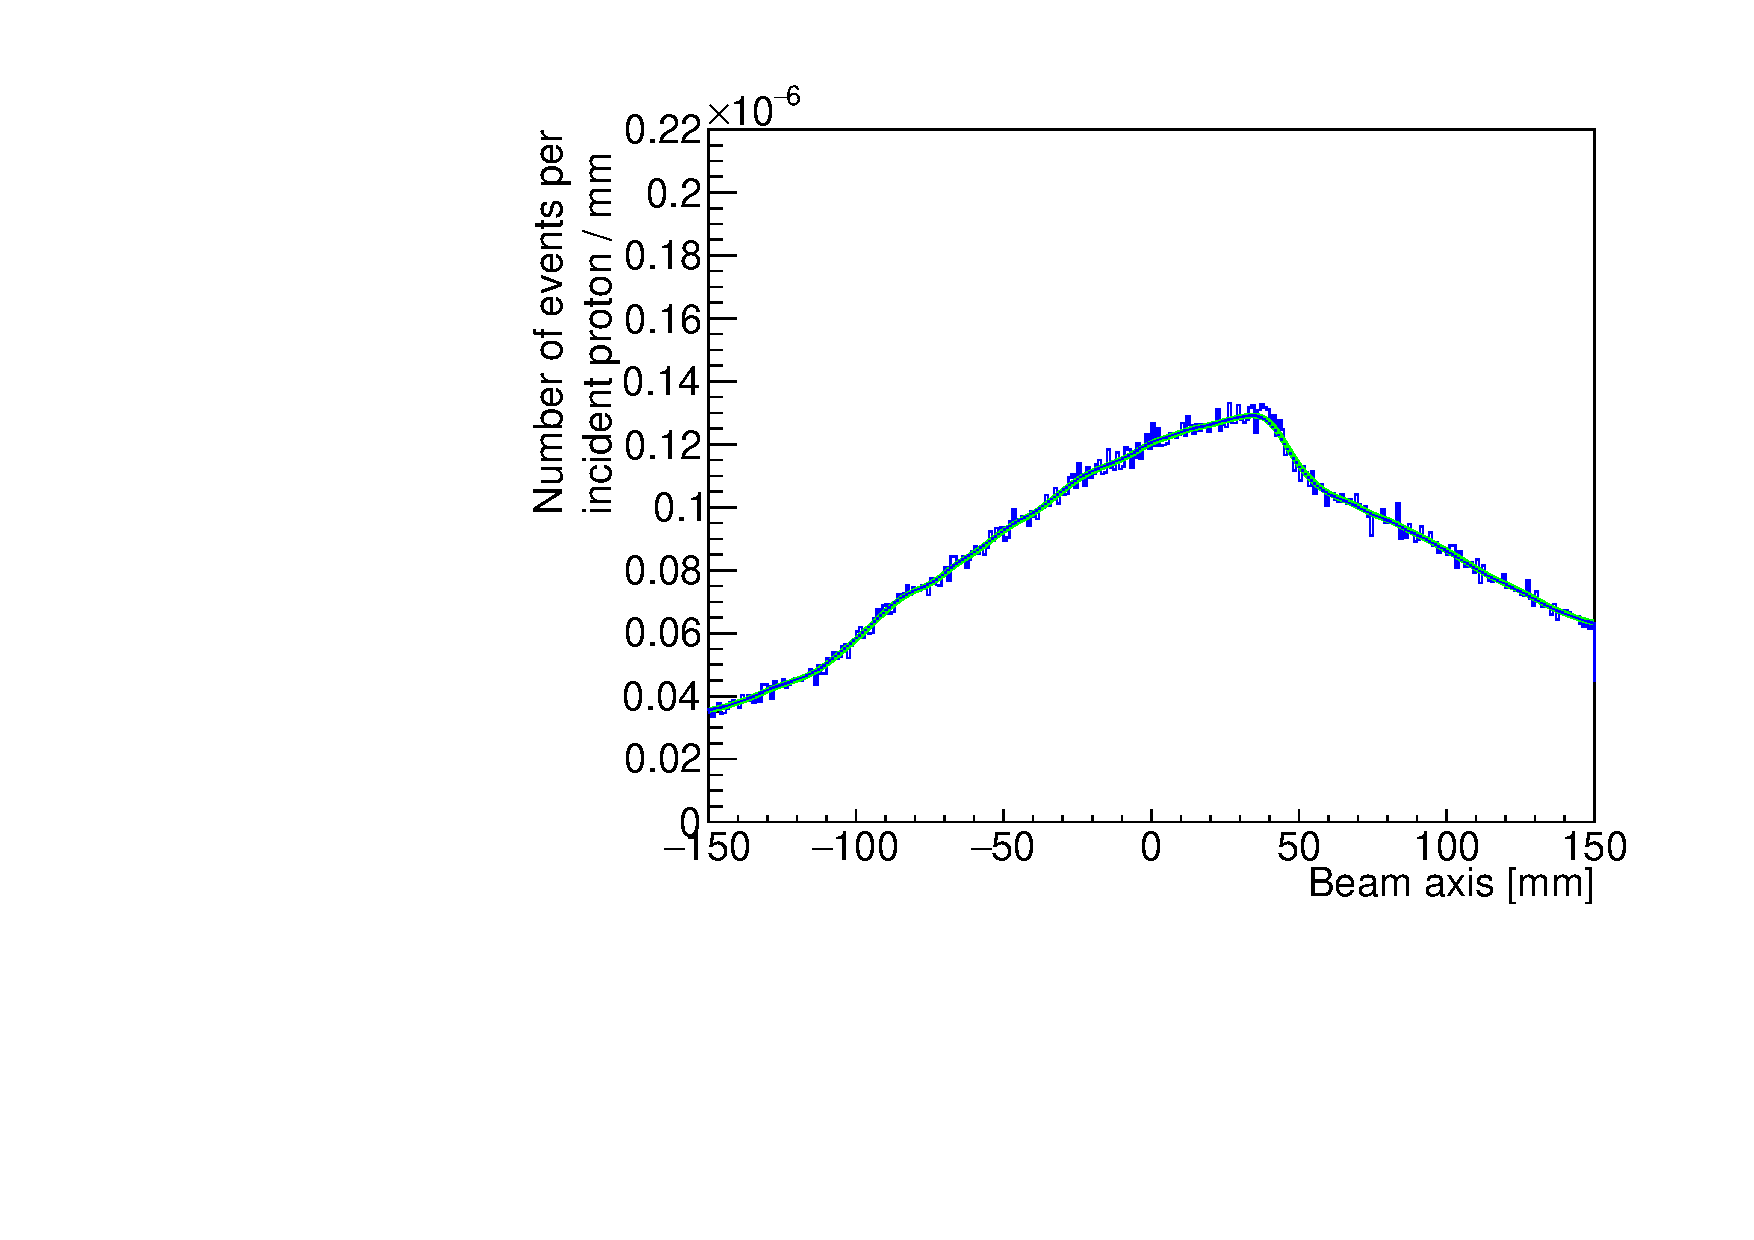
\includegraphics[width=0.9\textwidth]{03_GraphicFiles/chapter4_HTsimu/Results_forHadronthPaper/RefProfile_lineCone_plusNurbs.pdf}
\caption{}
\label{chap4::fig::fig_Results_Estimation_Camera_Profil_highStat_CC_simulation_Hadronth_LineCone}
\end{subfigure}
\begin{subfigure}[b]{.5\textwidth}
\centering
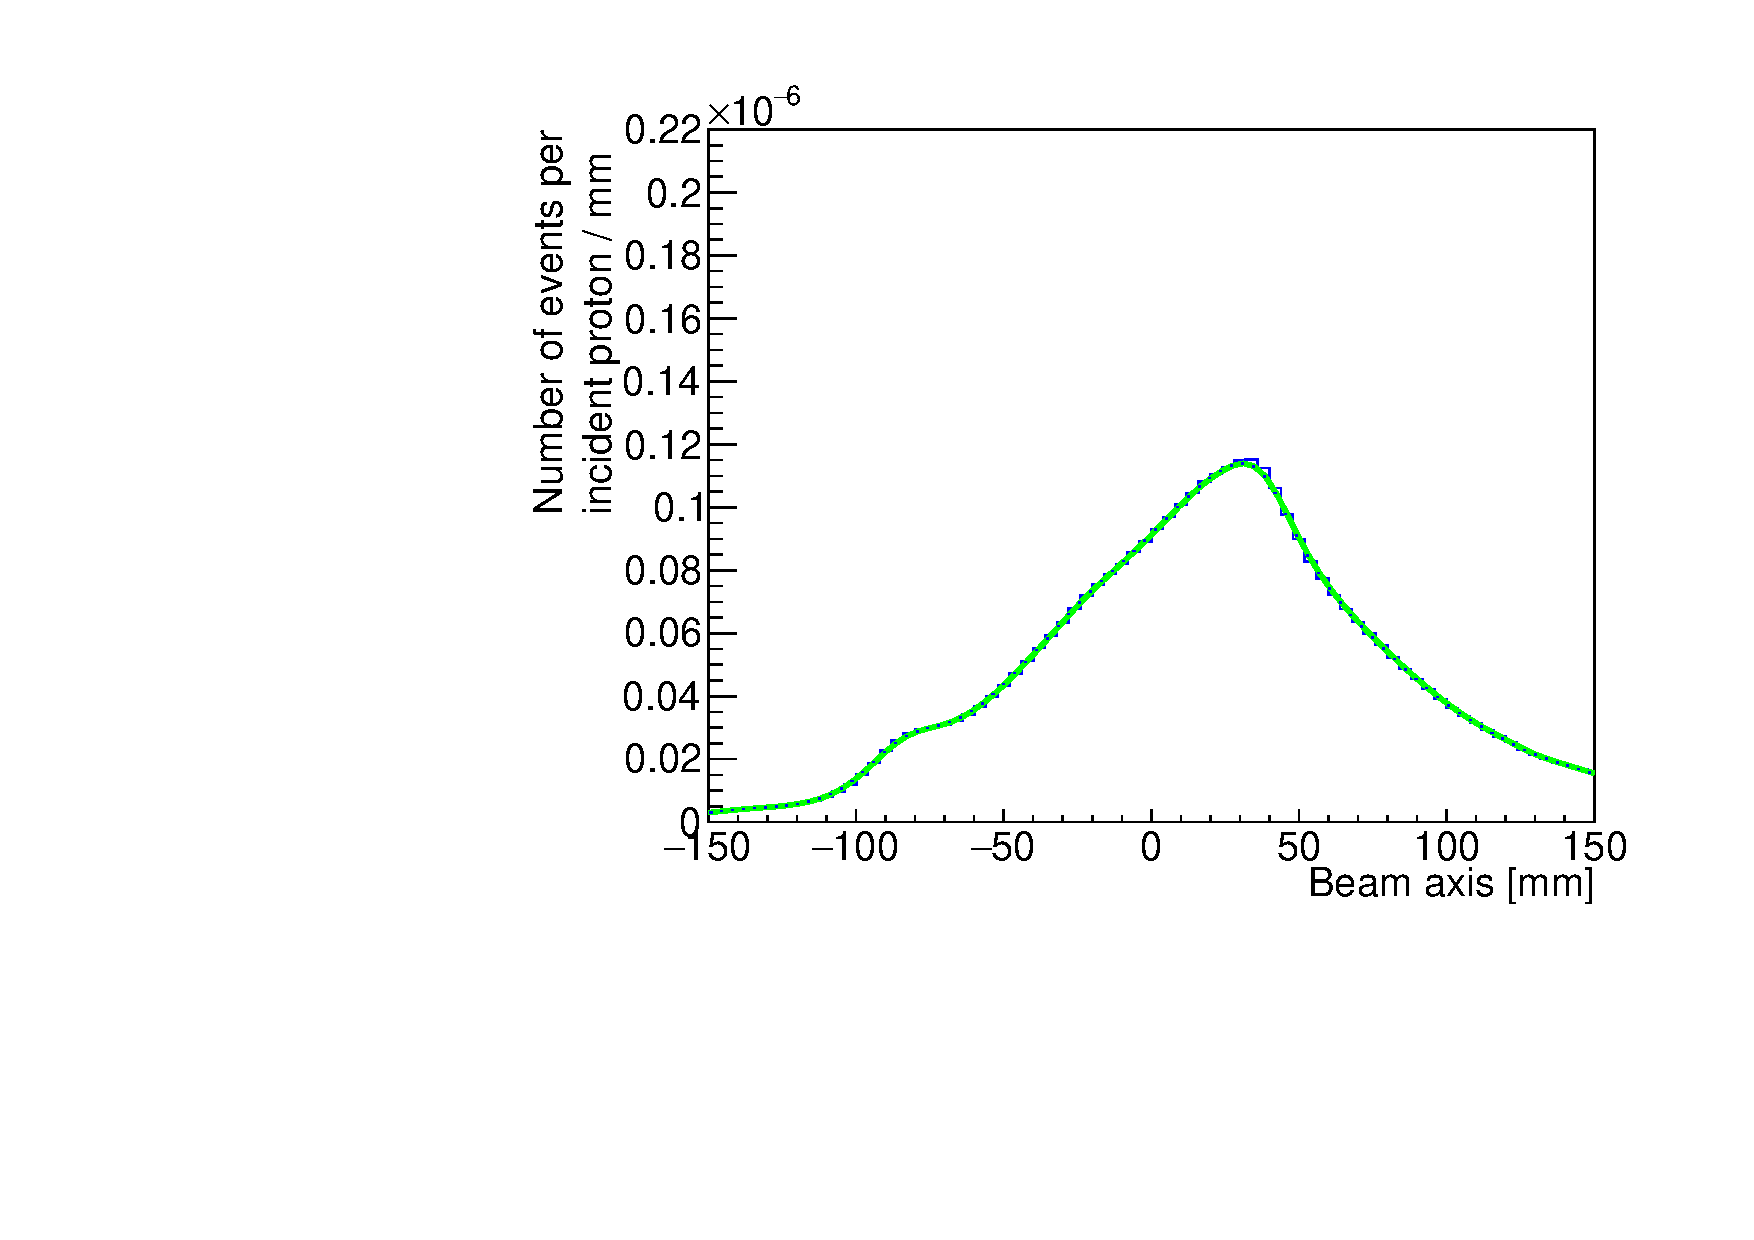
\includegraphics[width=0.9\textwidth]{03_GraphicFiles/chapter4_HTsimu/Results_forHadronthPaper/RefProfile_MLEM_plusNurbs.pdf}
\caption{}
\label{chap4::fig::fig_Results_Estimation_Camera_Profil_highStat_CC_simulation_Hadronth_MLEM}
\end{subfigure}
\begin{subfigure}[b]{.5\textwidth}
\centering
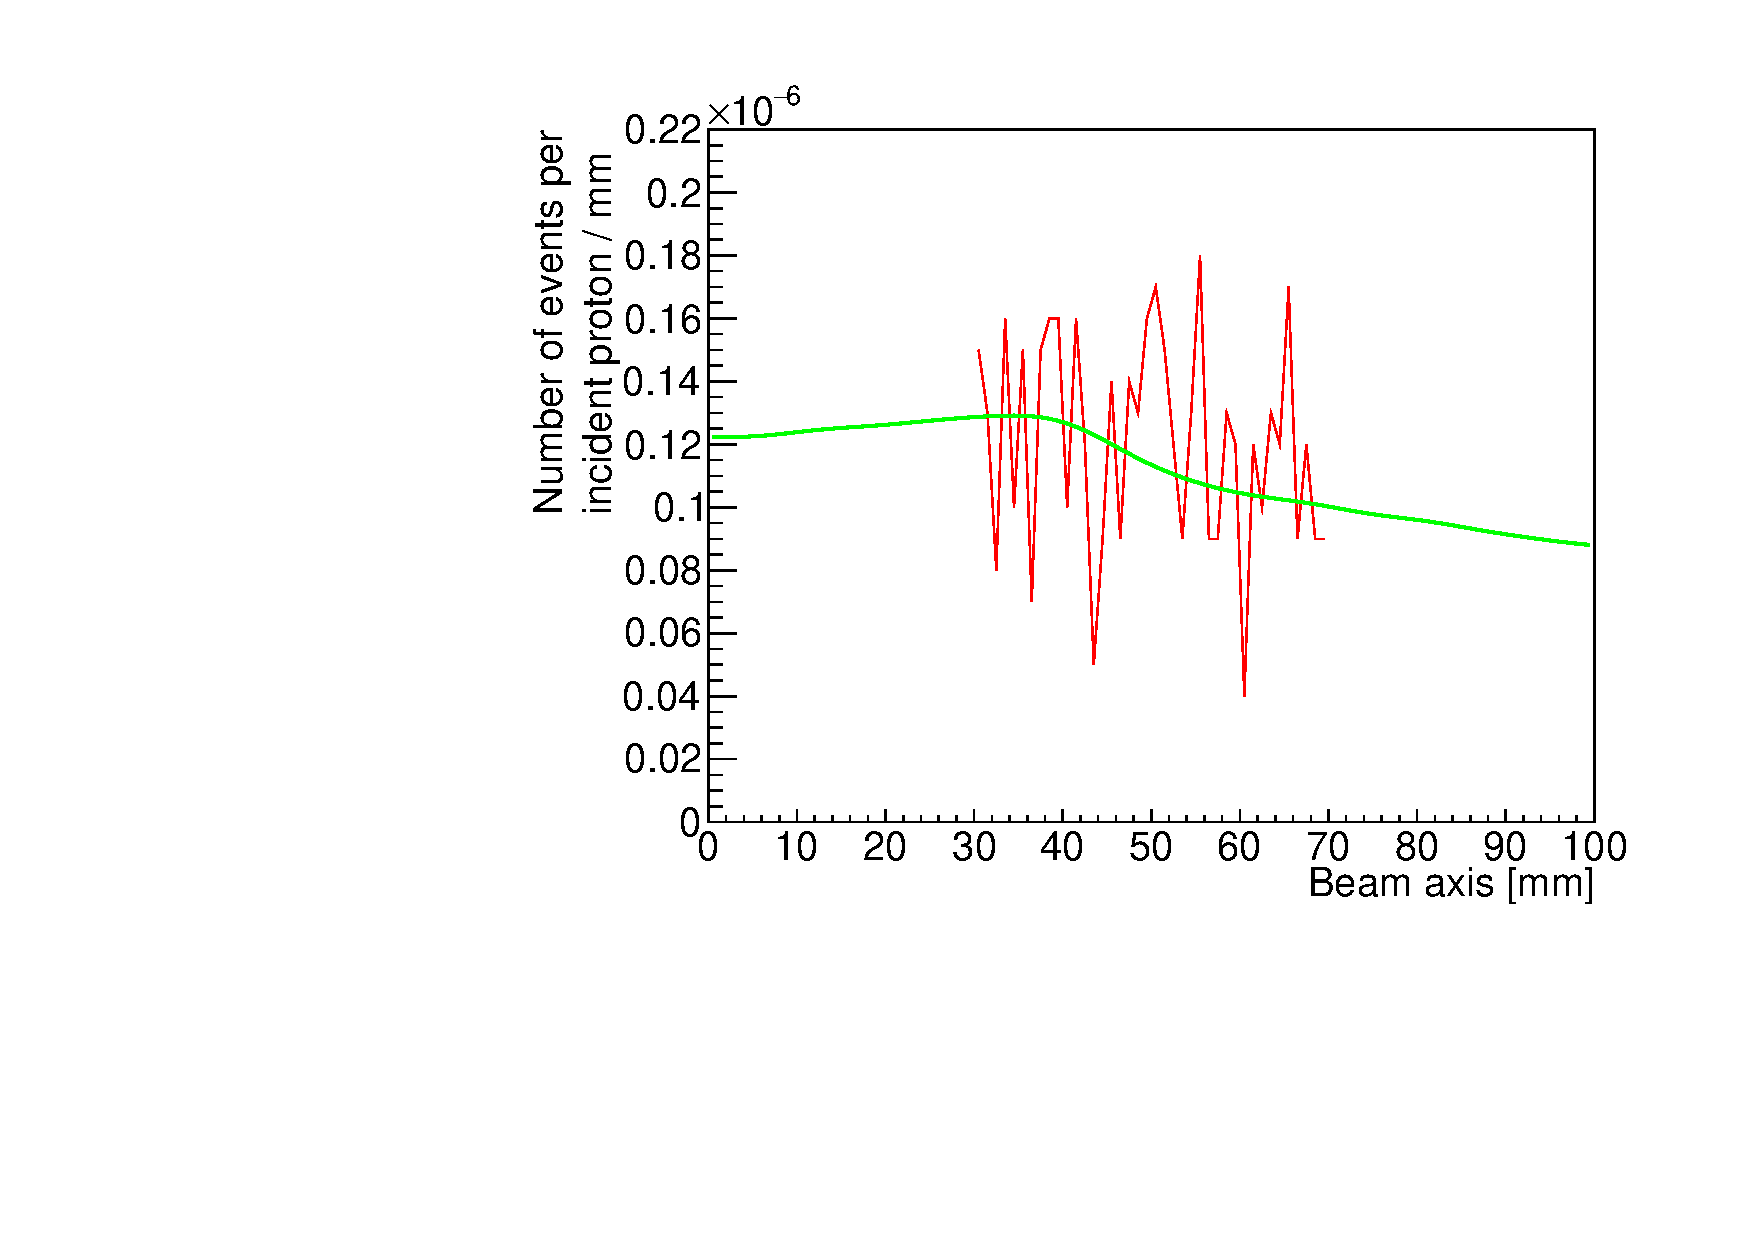
\includegraphics[width=0.9\textwidth]{03_GraphicFiles/chapter4_HTsimu/Results_forHadronthPaper/profile_Poisson_lineCone_green.pdf}
\caption{}
\label{chap4::fig::fig_Estimation_Camera_CC_NURBS_Poisson_LC}
\end{subfigure}
\begin{subfigure}[b]{.5\textwidth}
\centering
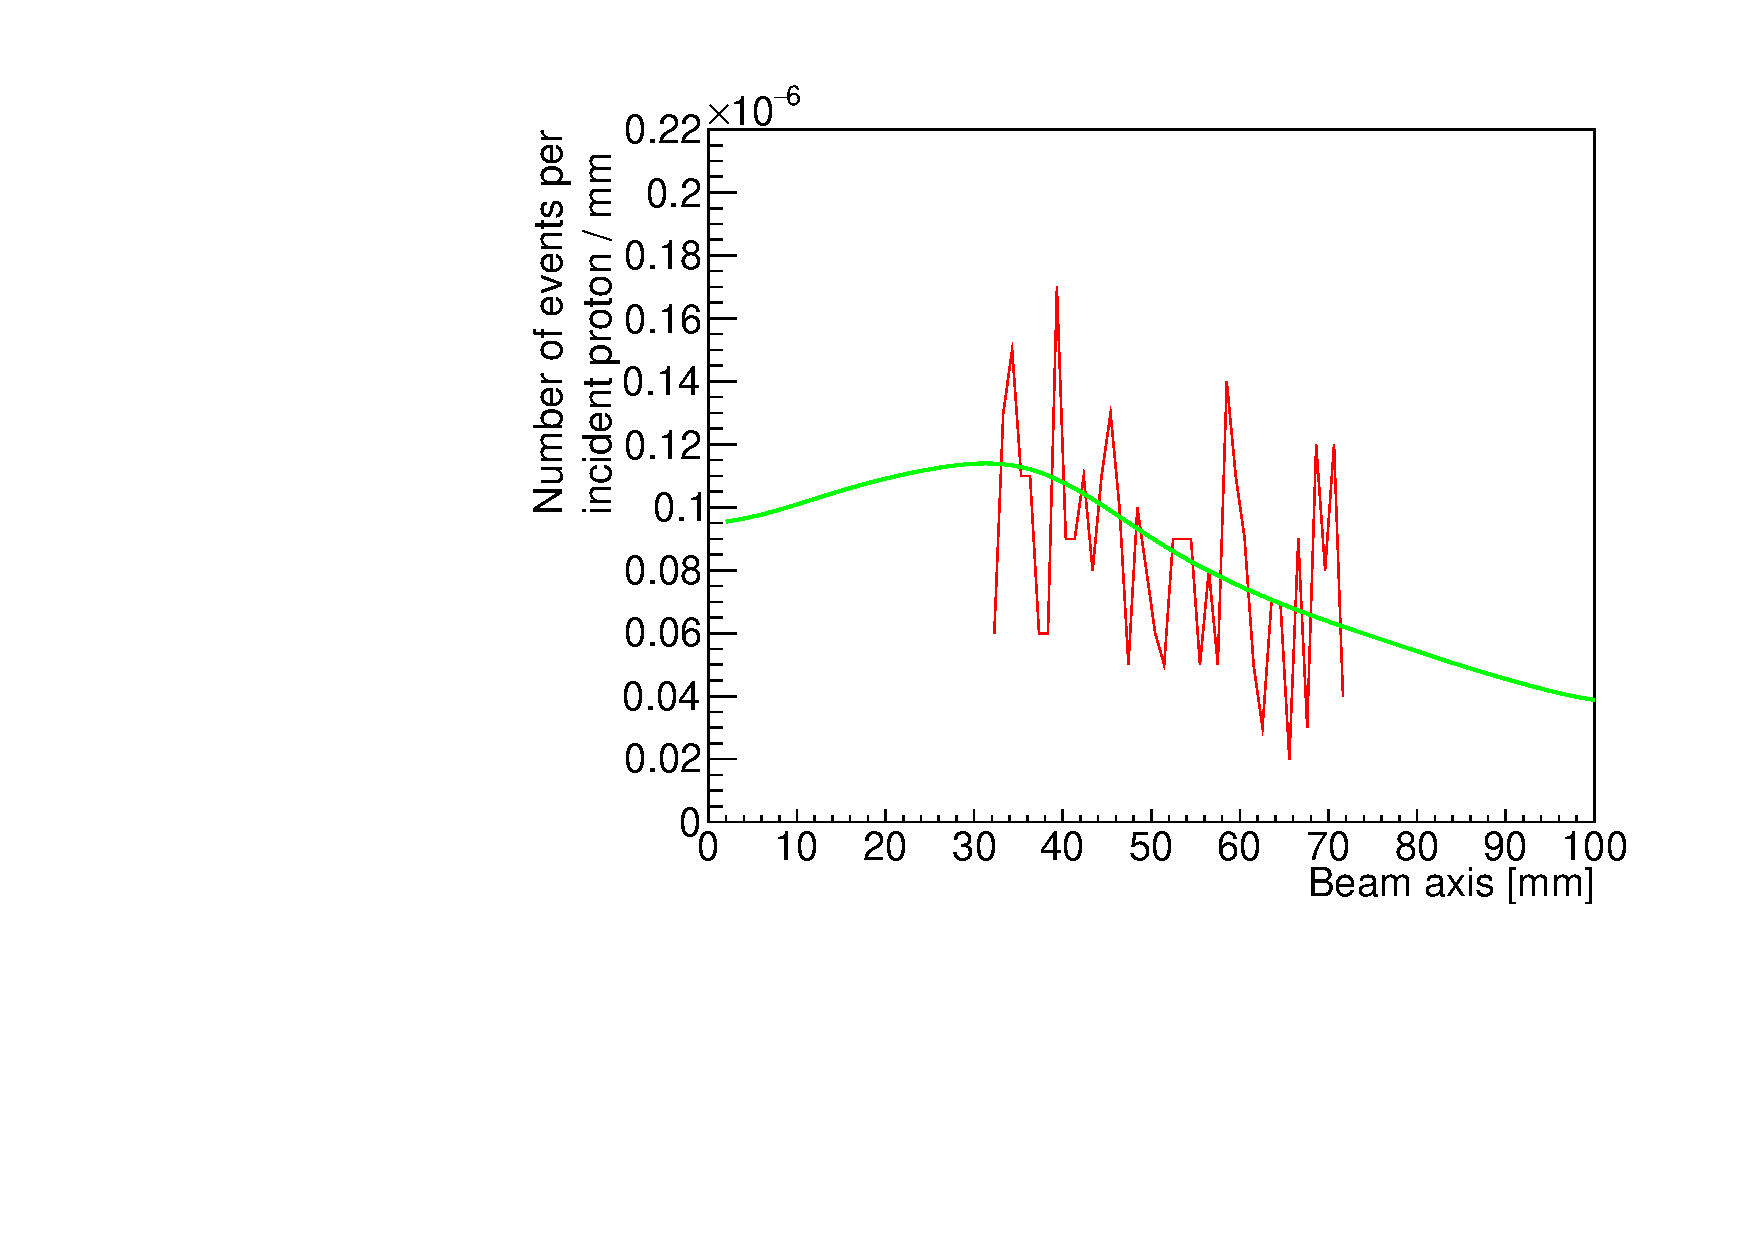
\includegraphics[width=0.9\textwidth]{03_GraphicFiles/chapter4_HTsimu/Results_forHadronthPaper/profile_Poisson_MLEM_green.pdf}
\caption{}
\label{chap4::fig::fig_Estimation_Camera_CC_NURBS_Poisson_MLEM}
\end{subfigure}
 \caption{Data processing comparison for the same proton simulation with the line-cone algorithm (left column) and the \gls{lm-mlem} algorithm (right column). The first row gives the reconstructed reference profile (blue histogram) for $10^{10}$ incident protons, at a beam intensity of 1 proton per bunch, with the \gls{nurbs} related curve (green solid line). The second row shows the \gls{nurbs} curve (green) obtained after the normalization to a $10^8$ incident protons statistics and the profile realization with the addition of Poisson statistical fluctuations (red); the curves are centered on the expected \gls{fop} at 50~mm. }
\end{figure}

\begin{figure}
\begin{subfigure}[b]{.5\textwidth}
\centering
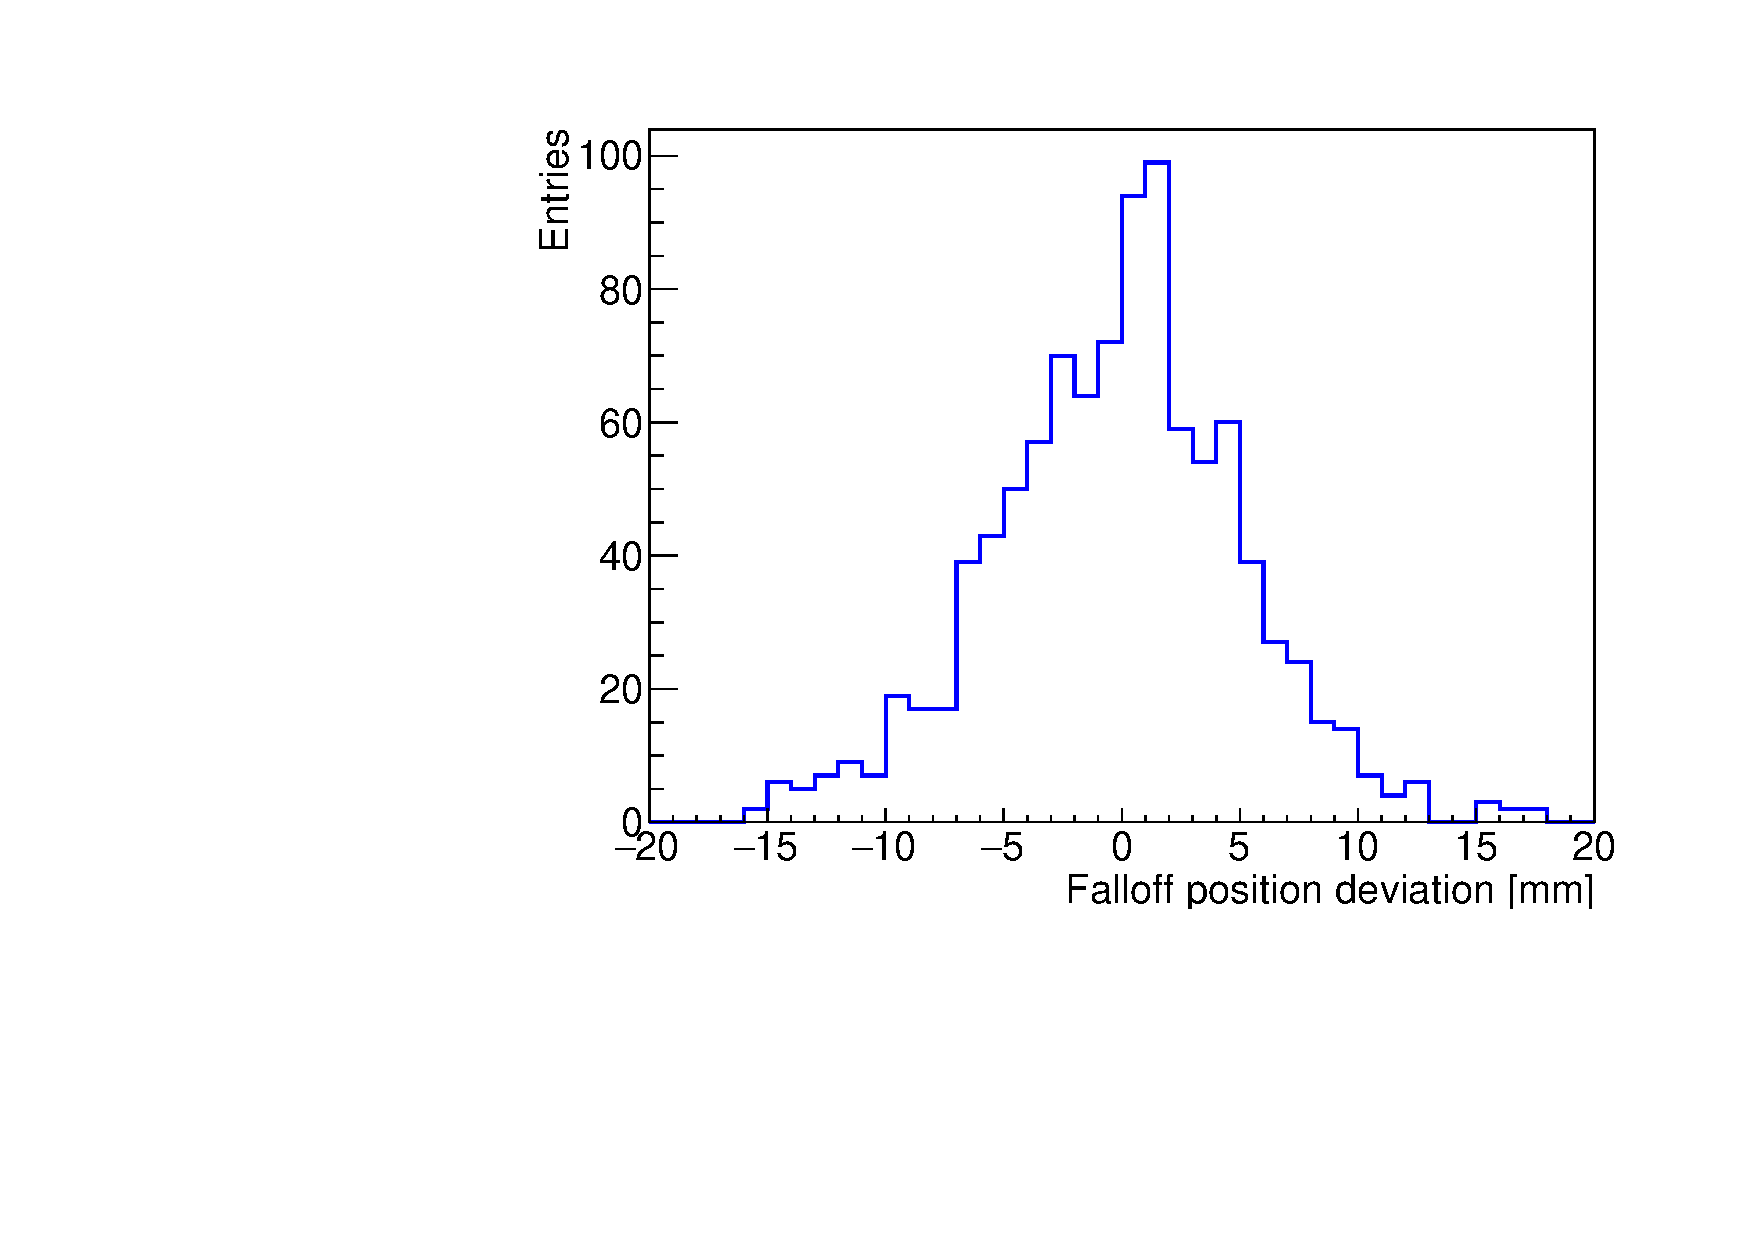
\includegraphics[width=0.9\textwidth]{03_GraphicFiles/chapter4_HTsimu/new/LC_histo_deviations.pdf}
\caption{}
\label{chap4::fig::fig_Results_Precision_Distribution_Variation_CC_simulation_Hadronth_LC}
\end{subfigure}
\begin{subfigure}[b]{.5\textwidth}
\centering
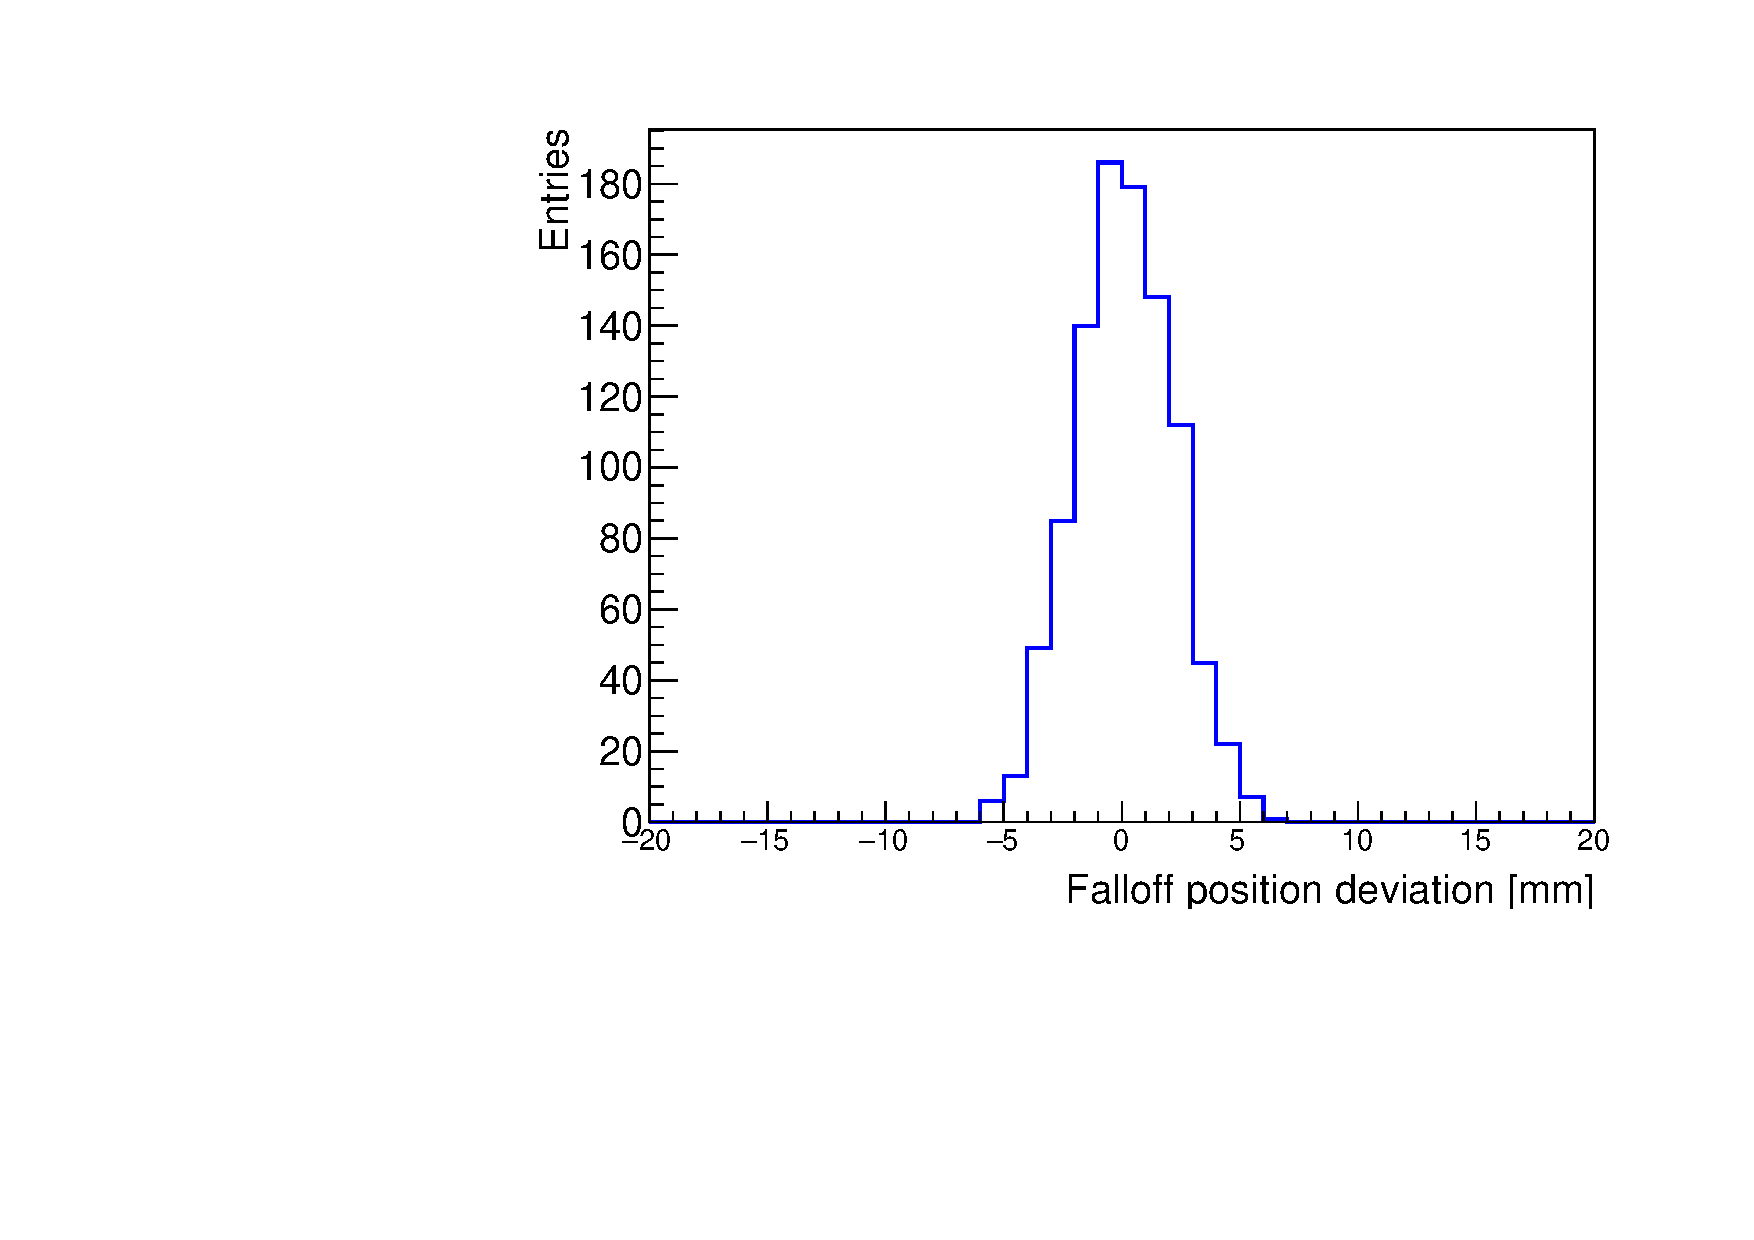
\includegraphics[width=0.9\textwidth]{03_GraphicFiles/chapter4_HTsimu/new/MLEM_histo_deviations.pdf}
\caption{}
\label{chap4::fig::fig_Results_Precision_Distribution_Variation_CC_simulation_Hadronth_MLEM} 
\end{subfigure}
\caption{Distributions of the fall-off position deviation with respect to the fall-off position of the high statistics reference profile for 1000 realizations with 10$^8$ primary protons, obtained with line-cone (a) and \gls{mlem} (b) reconstruction. The \gls{rms} of these distributions represents the Compton camera precision for the selected statistics.}
 \end{figure}

The analysis method described in section~\ref{chap4::subsubsec::MatMeth:precision} is applied to the different \gls{pg} obtained profiles to retrieve the camera precision in the fall-off identification. The results are shown in \figurename~\ref{chap4::fig::precision}, where the two reconstruction methods are represented by different markers.

\begin{figure}	
\centering
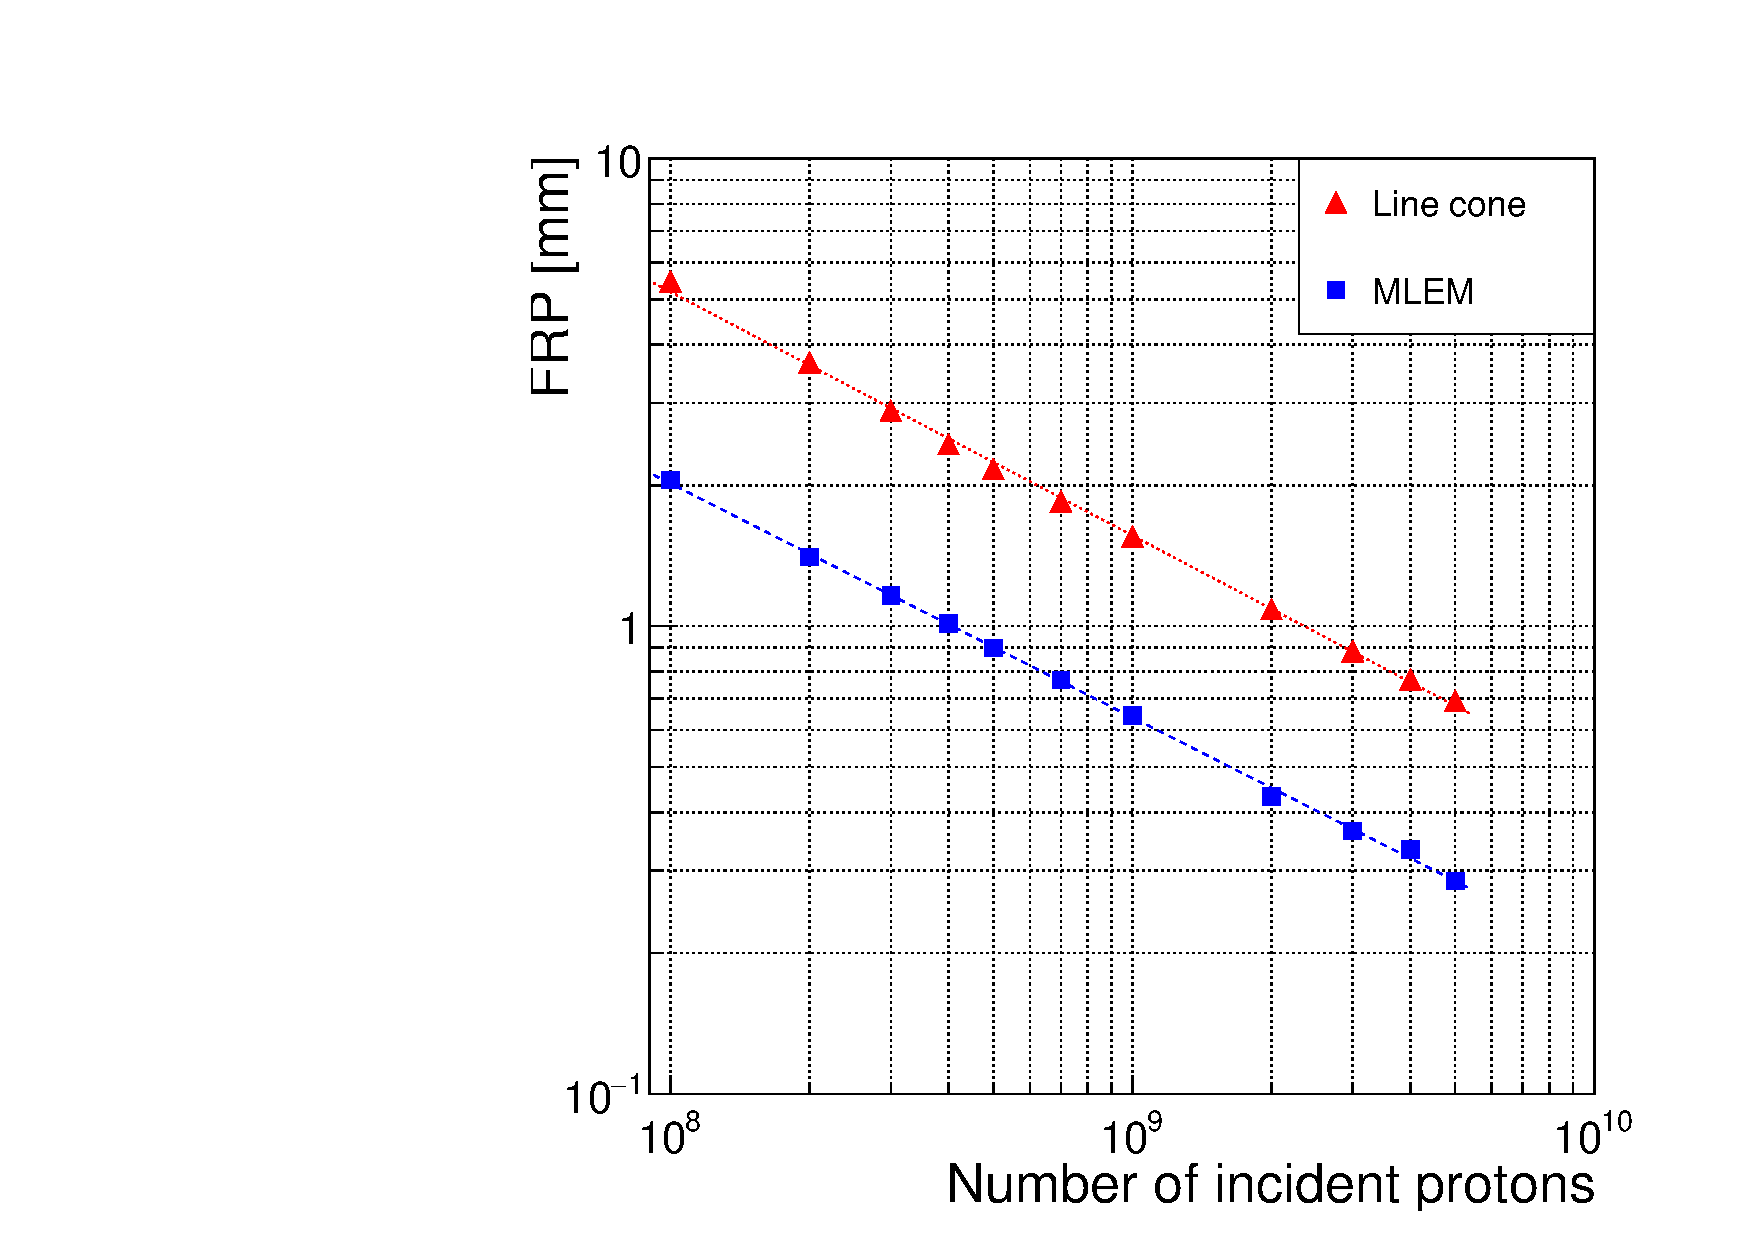
\includegraphics[width=0.6\textwidth]{03_GraphicFiles/chapter4_HTsimu/new/precisionVSprimaries.pdf}
\caption{\gls{frp} for two different reconstruction algorithms: line-cone and \gls{lm-mlem}. The precision is shown as a function of the total number of incident protons, in the range $1\times10^{8}$ to $5\times10^{9}$.}	
\label{chap4::fig::precision}
\end{figure}

The iterative \gls{mlem} reconstruction method enables one to achieve a better precision with respect to the line-cone algorithm: the \gls{frp} is improved by a factor between 2 and 3 in the whole range of statistics explored. A linear behavior, highlighted by the performed linear fit of the two data sets, is verified with increasing number of primary protons, starting from the single spot scale of about 10$^8$ primaries, till $5\times10^9$ protons, which can correspond to the monitoring of a group of spots with the same planned range. 

\section{Discussion}

We studied in this simulation work the performance of the \gls{clarys} Compton camera prototype and its possible implementation as \gls{pg} detector for ion beam therapy monitoring. The proposed analysis is focused on four main points: detection efficiency for various kind of coincidence events, and for events with a single scatterer layer hit absolute gamma detection efficiency, true and background coincidence rate and camera precision in the identification of the prompt-gamma emission profile fall-off.

The gamma detection efficiency has been measured with the detector exposed to gamma sources at six different energies, in the prompt-gamma energy range. The relative detection efficiency has been studied considering the three possible kinds of true coincidence events: single Compton interactions in the scatterer (2 photon interaction events), Compton recoil electron escape events and events with multiple gamma interactions in the scatterer (3 or more photon-interaction events). The coincidences composed of one single Compton interaction in one of the scatterer layers and an energy deposit in one single absorber blocks represent the majority of the collected events in the whole explored energy range. However, for energies above 1~MeV the amount of electron escape events becomes significant. Such kind of events can be ideally exploited in the reconstruction, and the selection can be based on tracking analysis (if the escaped recoil electron interacts in more than one scatterer layer). In the camera performance evaluation study, only single events have been selected as first approach for a feasibility study of the Compton camera application in ion range monitoring. 
All the results discussed in the following have been obtained with such an event selection.

The absolute camera efficiency variation as a function of the source position has been reported, with an ideal detector and with the application of detection energy thresholds in scatterer (50~keV) and absorber (100~keV). 
For low energies, below 2~MeV, the increased efficiency in the central section of the camera active surface - shown in \figurename~\ref{chap4::fig::effPos_noCut} - is linked to the increased relative number of photons approaching the camera with small angles. These photons are more likely undergoing Compton scattering with a reduced energy deposition, which is recorded by an ideal detector and rejected by the fixed energy threshold. The effect is all the more important as the primary gamma energy is limited, creating the peculiar energy dependence of the efficiency reduction observed in the results in \figurename~\ref{chap4::fig::effPos_noCut}.
Regarding the dependence of the efficiency on the Compton camera position, an accurate setup with respect to the expected Bragg peak position appears mandatory for the detection optimization.

The study of the signal-over-noise ratio as a function of beam intensity was performed (see \figurename~\ref{chap4::fig::coincidences}). The results show that, at clinical intensities, this ratio is very low. The \gls{tof} selection is effective in the case of carbon beams, where a significant proton and neutron contamination is expected. If we consider the case of proton beams, the amount of background and true coincidences is comparable at an intensity of about 1 proton per bunch, so that a clinical intensity reduction should be necessary to fit this configuration. The profile fall-off retrieval could not be achieved at clinical proton beam intensity for a single spot with the tested reconstruction methods. Even if a possible image reconstruction is not excluded by the low signal-over-noise ratio detected at realistic beam intensity with increased statistics (a group of spots with same expected range), given the fact that the background coincidences are distributed in an homogeneous way in the reconstructed volume, an intensity reduction can be an option in order to obtain more significant data sets. It must be noticed that the need for online check of Bragg peak position is all the more necessary for distal spots, which are in general the firsts to be treated, so that a beam intensity reduction at the beginning of the treatment can be foreseen in case an accurate monitoring is strictly needed. This would not affect the treatment delivery, nor the planned patient rate in the clinical work-flow; indeed, the spreading of the time duration for few spots is of the order of one second. 
In the case of carbon ions, the larger amount of secondary neutron produced during the patient treatment seems to require other background rejection methods in order to lead to an advantageous signal-over-noise ratio. Note also that online filtering strategies may be used to improve the quality of the data (see \figurename~\ref{chap4::fig::rate_full_abs}): already in \figurename~\ref{chap4::fig::coincidences}, one can notice that the amount of reconstructed events is about half that of true gamma, which means that partial absorption in the absorber leads to events which cannot be reconstructed via the line-cone method. More refined pre-analysis could be used and have been proposed in \cite{Draeger2017}. Note also that the line-cone reconstruction used here is quite rough: the two reconstruction points are systematically considered, although further selection may refine the procedure and improve the profile quality (for instance, rejecting points outside the planned treatment volume).
Alternative approaches for the optimization of the signal-over-noise ratio should be focused on the camera geometrical design. In~\cite{Fontana2017_APPB} we tested the same prototype with two absorber configurations, showing an absolute efficiency reduction of a factor approximately two when reducing the absorber from a $8\times6$ block matrix to a $3\times3$ one. Such a significant absorber size reduction is expected to drastically reduce the random coincidence contamination, thus improving the signal-over-noise ratio, with not dramatic efficiency degradation for the \gls{fop} monitoring purpose. Moreover, to this efficiency reduction corresponds an increased spatial resolution, probably given by the selection of gamma scattered with small angles. This hypothesis is confirmed by the efficiency variation generated by the applied energy thresholds, as discussed before. 
The design optimization could also foresee the reduction of the number of silicon layers, with a further expected reduction of the background coincidence rate. In addition to the aforementioned advantages, a more compact configuration allows for the implementation of several detector heads, which can be set at different angles and provide additional spatial information, in particular in view of three-dimensional imaging. In case the highest possible efficiency is required, the distance between scatterer and absorber can also be modified, knowing that for reduced distances the efficiency is increased because a minimal amount of scattered photons escapes the absorber field of view. On the other hand, a reduction of the inter-detector distance is not recommended for accurate \gls{tof} measurements (for fixed target-scatterer distance), given the uncertainty added by the detectors time resolutions. In addition to this, also the spatial resolution is affected by a reduction of the scatterer-absorber distance, given the increased amount of photons scattered with large Compton angles included in the collected events. Indeed, large angle scatterings tend to degrade the spatial resolution. Dedicated design studies will be performed in the next future to address the proposed improvements.  

The camera precision has been estimated for proton beams at the reduced intensity of 1 proton per bunch on average, starting from a reference prompt gamma emission profile obtained at high primary particle statistics ($10^{10}$), with the random extraction of 1000 data subsets per number of incident protons and applying a robust minimization algorithm to define the shift of the identified profile fall-off with respect to the reference one.
The camera precision in the fall-off identification rapidly increases for increasing primary particle statistics. A sufficiently good precision is achieved on a spot basis for proton beams, where the precision is about 2~mm with a \gls{mlem} reconstruction: a qualitative monitoring of each spot seems then possible. In order to achieve millimeter precision, some spot grouping methods must be considered, or multiple-head detector configurations, e.g in a ring geometry. As a general result, the \gls{lm-mlem} iterative algorithm, which is now the standard for this kind of image reconstruction, guarantees a better fall-off identification precision over the whole explored intensity range. However, \gls{mlem} does not exploit the additional information provided by the knowledge of the beam position in the transverse plane. In future studies, such a priori information should be considered in order to improve the reconstruction rapidity and image quality. In addition to this, more restrictive data selection during reconstruction can in principle improve the image quality and speed up the reconstruction process. At present, given the long calculation time required by the iterative algorithm, the line-cone reconstruction method can still be an option for on-line treatment check, when safety limit can be fixed in order to exclude severe deviation from the treatment planning and an interruption of the dose delivery in real time can be foreseen. Moreover, the \gls{tof} information can be included in the line-cone reconstruction method in order to constrain the emission on a single point, and improve its accuracy.
Finally, it should be noticed that the presented study is focused on events involving one single scatterer layer: the inclusion of electron escape events can increase the reconstruction accuracy, given the constraint imposed on the reconstructed surface by the electron tracking information. Further study is needed to assess the gain in precision provided by such kind of events. 

The Compton detection principle has already proven its potential in detecting prompt gammas for ion beam therapy monitoring purpose, and the \gls{clarys} Compton camera prototype shows promising results for this application. The detector is now at the final development stage, its components are being tested on beam in clinical facilities and a first beam test with a complete system is foreseen for the next year. New simulation studies are to be carried out to benchmark the Compton camera device to other detection systems, like \gls{pet} machines or collimated detectors, already used or tested in clinics for ion beam therapy monitoring. The proposed study verify the feasibility of range monitoring in particle therapy with the \gls{clarys} Compton camera with a minimal approach, and improved performance are expected after detector and reconstruction method optimization.            



\clearpage
%\printbibliography[heading=subbibintoc]
